\chapter{面向车联网的SDN架构以及编程框架}
\section{引言}

车联网(Internet of Vehicles,IoV)目前受到了学术界和工业界的巨大关注。通信技术和智能城市的巨大发展给IoV带来了更多可能的服务,提高了车辆驾驶的质量和安全性。为了IoV的进一步发展,目前已有多个研究和工业组织在实施各种相关项目~\cite{CVIS, makino2005smartway}。例如,欧盟领导的CVIS~\cite{CVIS}致力于发展车与车之间以及车与路旁设施之间的通信技术;Smartway~\cite{makino2005smartway}的目标是集成多个智能传输系统并提供一个统一的平台。

%Internet of Vehicles (IoV) is attracting considerable attention from both academia and industry. The vigorous development of communication technology and smart city makes various services possible in IoV, which significantly improves the quality and safety of human driving. Research and industry communities are carrying out several projects~\cite{CVIS, makino2005smartway} for the development of IoV. For example, EU's CVIS~\cite{CVIS} is committed to the development of the technologies needed to allow cars to communicate with each other and with the nearby roadside infrastructure. Smartway~\cite{makino2005smartway} focuses on integrating all intelligent transportation system functions to a uniform platform and provisioning services by two-way communications.

虽然IoV有着很好的发展前景,但其中网络设备的封闭性阻碍了IoV上新服务的快速部署和更新。网络设备(如交换机、路由器)目前由不同的厂商开发,设备的更改需要专业人员的手工配置,使网络管理变得昂贵并且易出错。由于缺少一个开放和统一接口,无法实现网络的灵活和动态的配置,从而影响大规模IoV上新服务的部署和拓展。为了IoV的发展,一个新的网络架构是必要的。

%Though there is a promising future in IoV, the proprietary and closed way of operating devices in networks slows down the deployment and extension of new services in IoV. Network devices such as switches and routers are developed by different manufacturers. Their changes require substantial manual configuration by trained operators, which makes network management expensive and error-prone. The lack of an open and unified interface for flexible and dynamically customizable networks makes it difficult to deploy and extend new services in large-scale IoV. A new network architecture is expected for the development of IoV.

关于新的网络架构以及下一代互联网,目前有如下相关的研究。命名数据网络~\cite{NDN}的目标为开发一个新的互联网架构。与传统互联网的从哪里获取服务相比,命名数据网络关注获取什么服务。为了实现移动过程中的无缝隙数据传输,MobilityFirst~\cite{MobilityFirst}将节点的移动性作为一个普遍场景进行设计。NEBULA~\cite{NEBULA}则设计了一个基于云计算和数据中心的新的网络架构。SDN将控制层和数据层进行了分离,并提供了配置网络的统一的接口。一个统一的配置网络设备的接口,使大规模可灵活配置的网络变得可行,从而可以加速IoV上新服务的部署。

%There are several projects for a new network architecture and next-generation Internet. Named Data Networking~\cite{NDN} aims to develop a new Internet architecture that concentrates on getting `what' services rather than `where' to get services. MobilityFirst \cite{MobilityFirst} supports seamless and smooth mobility. It takes the mobility of nodes as a common case rather than a special case in traditional networks. NEBULA \cite{NEBULA} develops a new network architecture based on cloud computing and data centers. Software-Defined Network (SDN) provides a unified interface to configure network equipment and separates a control plane from a data one. A unified interface of configuring network equipment makes a large-scale customizable network possible, and accelerates new service deployment in IoV.

考虑其开放和统一的接口,我们采用SDN作为IoV中底层网络架构,并提出软件定义车联网 (Software-Defined Internet of Vehicles,SDIV)的架构。除了其开放统一的接口,SDIV在以下方面有较大优势:1. 通过将控制平面和数据平面的分离,SDIV有着非常高的可拓展性;2. 通过逻辑上集中式的控制器,SDIV简化了网络的管理;3. SDIV中的控制器可以根据当前网络状况计算数据传输的最优路径并协调车与路旁电子设备之间的通信。

关于SDIV上的编程框架,由于车辆的移动性,我们提出将底层每一个交换机的数据通路分为两个部分:面向静态转发路径部分和面向动态转发路径部分。其中静态部分则由高级SDN程序编译生成(该部分不会随着车辆移动而变化)。对于动态部分,由于车辆的不断移动,提前生成流水线结构以及流表项并不是一个好的设计。因此SDIV将动态转发路径部分设计为单流表的响应式下发流规则。鉴于单流表的有限的流表容量以及IoV中的移动特性,如何构建紧凑的流表是SDIV的主要挑战,也是本章的主要技术内容。

%具体的应用可以是对

%由于SDIV的设计中,车辆的移动性是一个主要的考虑因素,该高级SDN程序中不会考虑数据包在全网的转发,而会处理一些本地的操作,如ACL等。对于面向全网络部分,由于车辆的不断移动,事先生成流水线结构以及流表项并不是一个好的设计,因此SDIV将面向全网络部分设计为单流表的响应式下发流规则。因此,对于这一部分,由于OpenFlow交换机的有限的流表容量以及IoV中的移动特性,如何构建紧凑的流表是SDIV的主要挑战,也是本章的主要内容。

%We adopt SDN to support IoV for its open and unified interface, and propose Software-Defined Internet of Vehicles (SDIV), a new architecture for the development of IoV. SDIV has several advantages in supporting IoV besides the open and unified interface: (1) it essentially has high scalability by separating a data plane from a control one, (2) it achieves desired network manageability by using a logically centralized controller, and (3) its controller is able to choose the best path for data transmission and plays as a coordinator for roadside electronic devices according to the current network state. However, IoV characteristics introduce challenges in rule (match and corresponding action) installation due to the limited size of flow tables in its OpenFlow switches. It is thus necessary to build compact flow tables for scalability of IoV.

本工作中,我们考虑IoV中的实时查询服务,来给出SDIV中优化的流规则设置细节。通过实时查询服务,驾驶员可以获取实时的道路或其他信息来选择正确的驾驶方向。道路信息来自于路旁的监控摄像头并传给有需求的车辆。在此场景中,具体问题如下:1. 由于车辆的移动,车辆和摄像头之间需要不断建立新的连接,从而增加了流规则的数量;2. 当车辆与多个摄像头进行连接时,由于它们具有相同的目的,对每一个连接设置流规则并不高效。图~ \ref{fig1}描述了上述的问题。如果控制器简单地对每一个请求都下发流规则,则交换机中流表容量会成为系统瓶颈,并最终影响实时查询服务的性能。

%In this work, we consider real-time query services, that are typical in IoV, to show the design details for improved rule installation in SDIV. Real-time query services provide drivers the real-time road and other information and drivers decide which way to go according to such information. Road information coming from the surveillance cameras (or other kind of roadside electronic devices) is transmitted to every vehicle with demanding. In this scenario, the specific issues are: (1) the mobility of vehicles increases the number of rules since it needs to establish new connections between vehicles and surveillance cameras, and (2) when a vehicle is connecting to multiple cameras, it is not efficient to install rules for every path since it has the same destination. Fig. \ref{fig1} illustrates the issues of rule installation in IoV. If the controller simply installs rules upon the request of drivers, the table size at switches may become the performance bottleneck of a real-time query service in IoV and even fail the service.

\begin{figure} [t]
\begin{center}
\begin{tabular}{cc}
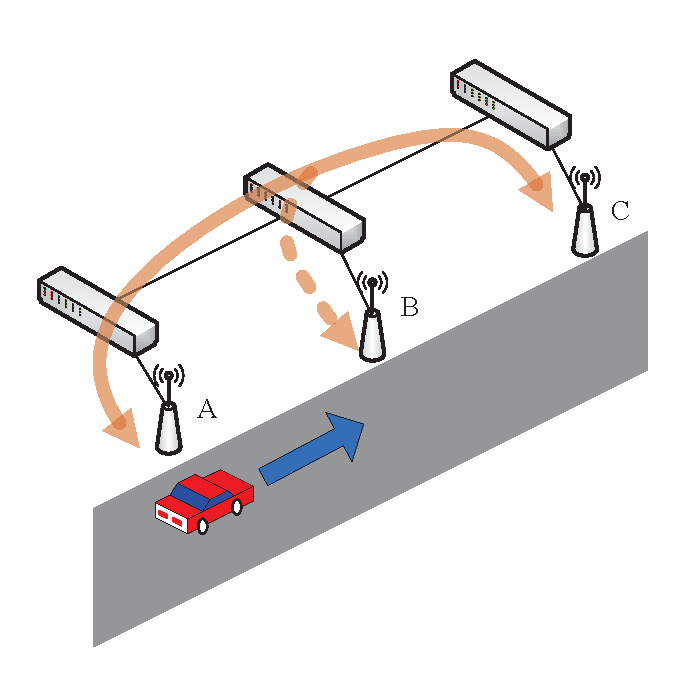
\includegraphics[width=0.48\columnwidth]{figures/fig-1-a-28.eps}&
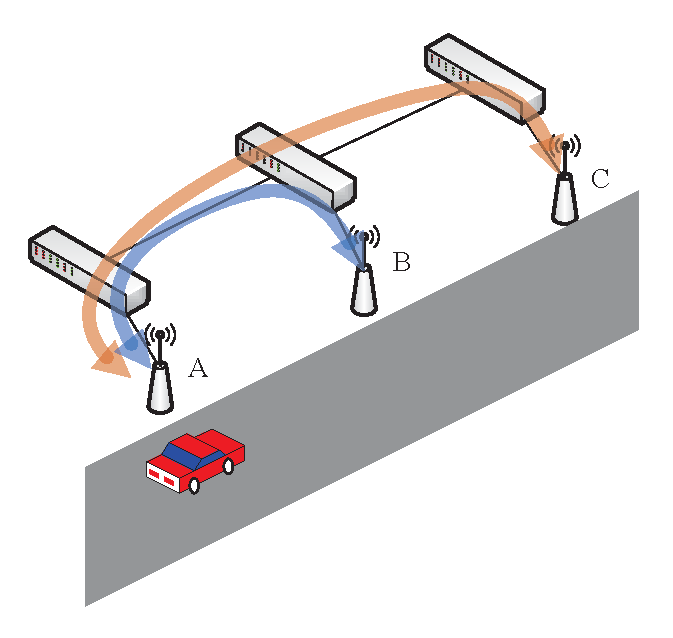
\includegraphics[width=0.48\columnwidth]{figures/fig-1-b-28.eps} \\
(a) & (b)
\end{tabular}
\caption{(a): 当车辆从$A$移到$B$时,它需要重新建立连接。虚线表示连接尚没建立;(b)当车辆同时连接多个摄像头时,对于每个连接建立路径下发规则并不高效由于所有的路径目的一样(即所有数据流目的地址为$A$)。} \label{fig1}
  \end{center}
  % \vspace{-0.3in}
\end{figure}

为了解决实时查询服务中流规则设置问题,通过借助SDN的集中式细粒度的流控制,我们提出了以下技术:1. 为了减少车辆发出的请求数量,我们在数据从摄像头到车辆的最后一跳时采用多播地址;2. 为了保证在车辆移动过程中数据传输不会中断,我们根据车辆的行驶状况提前在交换机中设置流规则;3. 为了减少流规则数量以及保证数据传输的正确性,我们在分支节点更改数据包头。

%To address the rule installation and table size growth problems for real-time query services, we develop several techniques by leveraging the centralized and fine granularity of data flow control in SDN for improved rule installation: (1) To reduce the number of requests sent by vehicles, we use multicast addresses instead of general destination address as the last address when vehicles receive data from cameras; (2) To keep uninterrupted connection between vehicles and roadside electronic devices, we install rules in switches in advance based on the conditions of vehicles; and (3) To decrease the number of rules and maintain the correctness of data transmission, we modify the headers when packets come to branching nodes.
%



%In this paper, we first describe the SDIV architecture. We then analyze the problem of flow table size growth in OpenFlow-supported switches. We design and develop an optimization approach to reduce the number of rules in switches. We validate the feasibility of improved rule installation by considering four situations in a real-time query service and analyze the details of data transmission in each case. Finally we use Floodlight~\cite{Floodlight} as a controller and Mininet~\cite{mininet} as a testbed to evaluate the performance of our improved rule installation  method with a real data trace. Experimental results show that when using improved rule installation, the flow table in switches is more compact than simply installing rules without compromising the performance of data communication for real-time query services.
%
%The rest of the paper is organized as follows. In Section~\ref{Related Work}, we review related works. In Section~\ref{Architecture}, we introduce the SDIV architecture. In Section~\ref{Rule Optimization}, we discuss the improved rule installation issues and the proposed solution. We conduct extensive experiments and report results in Section \ref{Evaluation}.  We conclude the paper with future work in Section~\ref{Conclusion}.

\section{相关工作}

目前IoV中的大多数服务,例如,道路安全、车辆管理、车辆导航等,依赖于车与车(V2V)之间的数据传输以及车与设备(V2I)之间的数据传输~\cite{du2015information}。已有一些研究工作验证了通过路旁AP以及WiFi提供数据的连通性~\cite{ott2005disconnection, balasubramanian2008interactive}。

%Most applications and services in IoV, e.g., road security, fleet management, navigation, billing, and multimedia, rely on data transfers between vehicles and roadside infrastructure (V2I) and among vehicles (V2V) \cite{du2015information}.
%Several researches \cite{ott2005disconnection, balasubramanian2008interactive} have demonstrated the feasibility of providing connectivity via road-side APs and the ubiquity of WiFi.


% TODO XXX
Hare等人~\cite{hare2012policy}设计一个集中式的策略框架来管理车辆网络的光谱资源来保证用户需要的数据传输性能。Wu等人~\cite{wu2013improving}结合GPS信息提高了对车辆姿态估计的准确度。Ahn等人~\cite{ahn2012risa}第一个提出了面向车辆网络的分布式路面状况探测以及数据分发的架构。Calafate等人~\cite{calafate2012efficient}研究通过计算最优数据包大小以及决定最优前向纠错,实现广播下的可靠数据传送机制。

%The studies \cite{joshi2011vehicular, xu2011utilizing} deal with the efficient communication between APs and vehicles. For routing and data forwarding, \cite{sahu2015bang, zhang2014geomob, zhu2013zoom, nzouonta2009vanet} study the routing protocol and fast forwarding. Routing in IoV in different categories is well reviewed in \cite{cheng2015its}. To manage vehicular networks, a centralized policy framework is introduced and called Virtuoso in \cite{hare2012policy}. It manages spectrum resources while ensuring users to have suitable access to meet their communication needs. In \cite{abadi2015traffic}, traffic flow prediction for traffic forecasting and congestion management is made. The work \cite{wu2013improving} estimates the attitude of a vehicle for low-cost inertial navigation system/GPS. Ahn et al. \cite{ahn2012risa} present the Road Information Sharing Architecture (RISA), representing the first distributed approach to road condition detection and dissemination for vehicular networks. \textcolor{blue}{Calafate et al. \cite{calafate2012efficient} study reliable data delivery through broadcasting by computing the optimal packet size and determining the best Forward Error Correction (FEC) scheme.}

Grassi等人~\cite{grassi2014vanet}通过将命名数据网络应用于车辆网络中,实现了所有计算设备上的互通。并且设备的互通独立于它们以何种方式连在一起,如有线网路,ad-hoc网络,或延迟容忍网络。Yap等人~\cite{yap2010blueprint}通过将网络服务与底层设施的分离,提出OpenFlow无线网络以实现任何无线设施之间的互通。

%To establish a new architecture in vehicular networks, Grassi et al. \cite{grassi2014vanet} apply Named Data Networking to networking vehicles and enable networking among all computing devices independent of whether they are connected through wired infrastructure, ad hoc, or intermittent Delay Tolerant Network. Yap et al. \cite{yap2010blueprint} present an OpenFlow \cite{mckeown2008openflow} wireless network to achieve a free travel between any wireless infrastructures by separating the network service from the underlying physical infrastructure.

Kim等人~\cite{kim2013improving}考虑在校园网络以及家庭网络中利用SDN优化网络的管理。Kanizo等人~\cite{kanizo2013palette}提出一个分布式的框架对较大的交换机流表进行分解来应对交换机流表容量受限问题。Voellmy等人~\cite{voellmy2013maple}设计Maple系统来发现可重用的转发策略并通过一个踪迹树的结构记录对数据包的操作来减少下发的流规则数量。

%Software-defined network (SDN) is applied to improve network management in \cite{kim2013improving}. A distribution framework is proposed for decomposing large switch tables into small ones to handle limited-size switch tables \cite{kanizo2013palette}, which reduces the flow table size. Voellmy et al. \cite{voellmy2013maple} introduce Maple to discover reusable forwarding decisions and reduce the number of rules by a trace tree structure that records the access to a specific packet.

从以上讨论可以看出,虽然目前有很多IoV的研究工作以及相关的SDN的应用,但并没有考虑新服务的部署以及通过集中式的控制器优化IoV中数据传输。因此,我们提出SDIV的架构。

%From the above discussions, we can find that though there are many approaches for IoV development as well as various applications of the SDN concept, there is no or little work of the new service deployment and centralized management in IoV. Thus, we provide an SDIV architecture to do so.

\section{SDIV架构以及工作流程} 

本节中,我们首先给出SDIV架构,并通过实时查询服务来说明其工作流程。

%In this section, we propose an SDIV architecture and discuss its utility through a real-time query service in IoV. Before introducing it, we describe the basic SDN model and its main features.

\subsection{SDIV架构}

如图~\ref{fig2}所示,我们提出的SDIV网络是一个具有三层的架构。从下至上分别为,物理层,控制层,以及应用层。

%Our proposed SDIV network has a three-tier architecture. From bottom to top, it has physical, control and application layers, as illustrated in Fig. ~\ref{fig2}.

\subsubsection{物理层}

物理层包括车辆,接入点(Access Point,AP),路边电子设备,交换机,以及服务器(区别于SDN中的控制器)。车辆作为移动的节点通过附近AP与服务器进行连接。这里我们假设AP的数量足够多并可以覆盖所有道路。路边电子设备如摄像头收集完路况信息后需要将数据传送到服务器或车辆。交换机连接着AP,摄像头以及服务器。当收到车辆发送的请求时,服务器会将相应的信息传送给车辆。一辆车可以同时连接多个服务器。

关于交换机数据通路设计,如图~\ref{fig:sdiv-dp}所示。我们提出将每一个交换机的数据通路分为两个部分:面向静态转发路径部分和面向动态转发路径部分。其中静态部分则由高级SDN程序编译生成。该部分具体的应用可以是:IoV中设施之间的通信(如摄像头到服务器)或实现对数据包的非全网路由的操作(如ACL)。对于面向动态转发路径部分,由于车辆的不断移动,提前生成流水线结构以及流表项并不是一个好的设计。无法提前生成流表项可以很好理解,因为节点的移动性,流表项应该不断变化。对于流水线方面,由于车辆的不断移动,若对动态转发路径部分使用流水线结构,则要求网络中所有节点都为相同的流水线结构。该做法既浪费网络资源,也会增加数据包时延,因为数据包经过流水线的时间与流表数量成正比。因此SDIV将面向动态转发路径部分设计为单流表的响应式下发流规则。

\begin{figure} [t]
\begin{center}
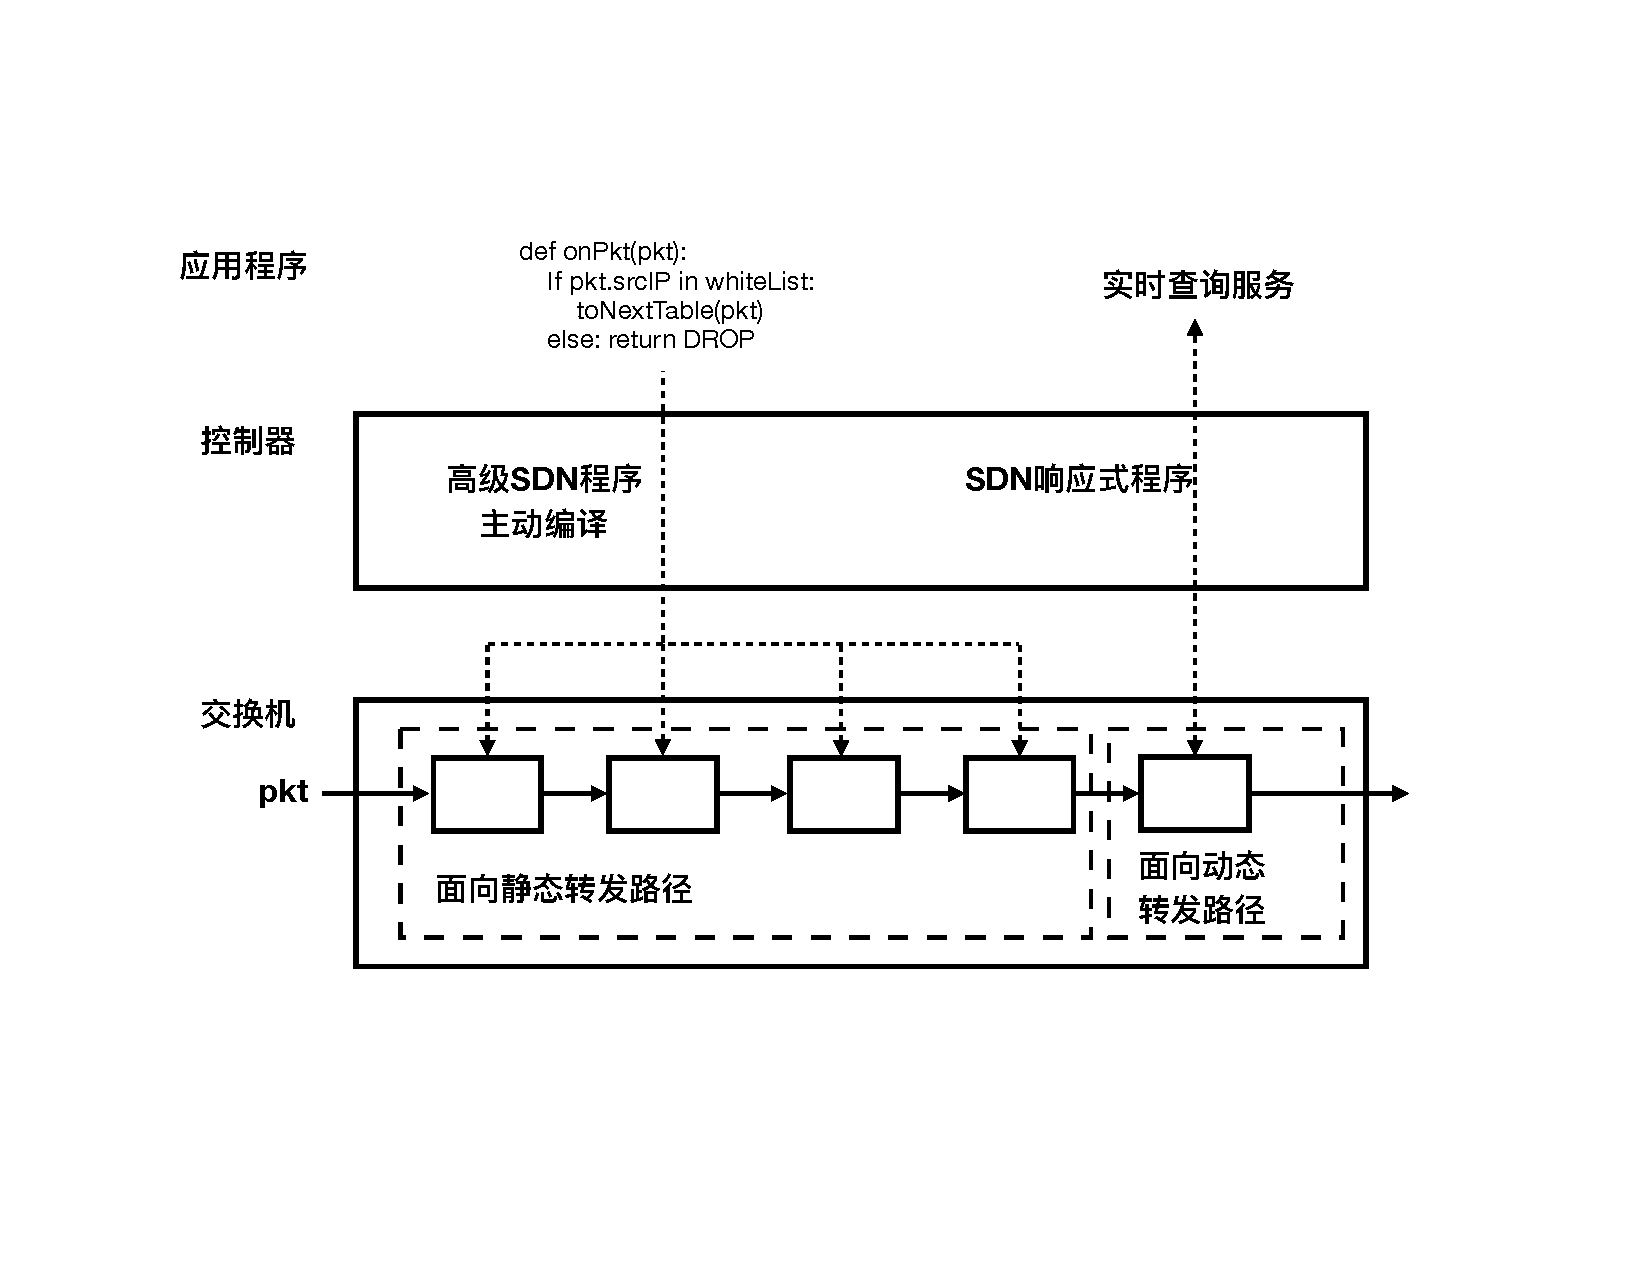
\includegraphics[width=0.8\columnwidth]{figures/sdiv-pf.pdf}
% \vspace{-0.2in}
\caption{SDIV的数据通路架构以及编程框架。} \label{fig:sdiv-dp}
\end{center}
% \vspace{-0.3in}
\end{figure}


%Physical layer includes vehicles, access points (APs), roadside electronic devices, switches, and servers (different from an SDN controller). Vehicles act as mobile nodes and communicate with the server through road-side APs. When sensors in a vehicle collect conditions of the vehicle, e.g. speed, direction and location, the data should be transmitted to the server as soon as possible. Vehicles receive responses from the server through nearby APs. Note that we assume that the number of road-side APs is sufficient to cover every road. Road-side APs are static WiFi APs reachable from \textcolor{blue}{the road that offers} the capability of data transmission to vehicles. Roadside electronic devices like surveillance cameras gather road conditions and also send data to servers or vehicles. Switches connect APs, surveillance cameras and servers. Servers here provide information service to vehicles, such as road conditions, based on the requests from vehicles and data collected from roadside electronic devices. One vehicle can connect to multiple servers at the same time.

\subsubsection{控制层}

利用SDN技术,控制层中的控制器连接着网络中的每一个交换机(包括AP)。通过下发OpenFlow流规则,控制器可以控制IoV中数据的传输。当网络状态发生改变时,交换机会发送相应的消息至控制器,使其获取最新的全局网络状态。通过全局网络状态信息,控制器可以将上层应用的策略,如路径选择或接入控制,转化为特定交换机上的OpenFlow流规则。

如图~\ref{fig:sdiv-dp}所示,对于面向静态转发路径部分,控制器支持通过主动式静态编译的方式将上层的高级SDN程序转化为底层数据平面的配置;对于面向动态转发路径部分,控制器采用响应式模式。

%In the control layer, the controller connecting to every switch (including APs) acts as a mediator between upper layer applications and underlayer network through SDN. By using OpenFlow, it is able to control all data flows in IoV. Also when the network state changes, the switches (including APs) notify it. In SDIV, they act as a connector among vehicles, servers and other roadside electronic devices by forwarding data flows based on rules which are installed by the controller. Then the controller can convert the strategy of application, e.g., the path selection or access control, into the OpenFlow rules in particular switches, since it has an up-to-date, global view of the network topology and traffic flows. The global network view makes the controller available to provide a customized network state to applications, which is not \textcolor{blue}{possible} in the traditional network. By this means, different applications have different views which benefit both applications and network. The former can have a much simpler view of the network than the detailed, but unnecessary view of the whole network, which can simplify their tasks, e.g., traffic scheduling. For the later, privacy and security benefit from the customized network state which guarantees the former to access their needed data only instead of all data.

\subsubsection{应用层}

所有的IoV应用程序组成了SDIV应用层。应用程序复杂给IoV中的车辆提供服务,如实时查询服务,位置服务等。每个应用从控制层的控制器中获取网络信息,并根据自身策略进行决策。

如图~\ref{fig:sdiv-dp}所示,对于面向静态转发路径部分的高级SDN程序可以直接转化为底层数据平面的配置;对于面向动态转发路径部分,则使用响应式模式进行开发。
%
%The strategy of each application is defined in the application layer. Applications provide services for vehicles in IoV, such as a real-time query service, location service and road information service. Each application gets the customized network state from the control layer and makes decisions according to its strategy. The strategy here instructs how to provide services to vehicles. A real-time query service example is to provide drivers the real-time conditions of roads. The network topology is required to compute the path for improving performance, which we will discuss later in Section~\ref{Rule Optimization}.
%

\begin{figure} [t]
\begin{center}
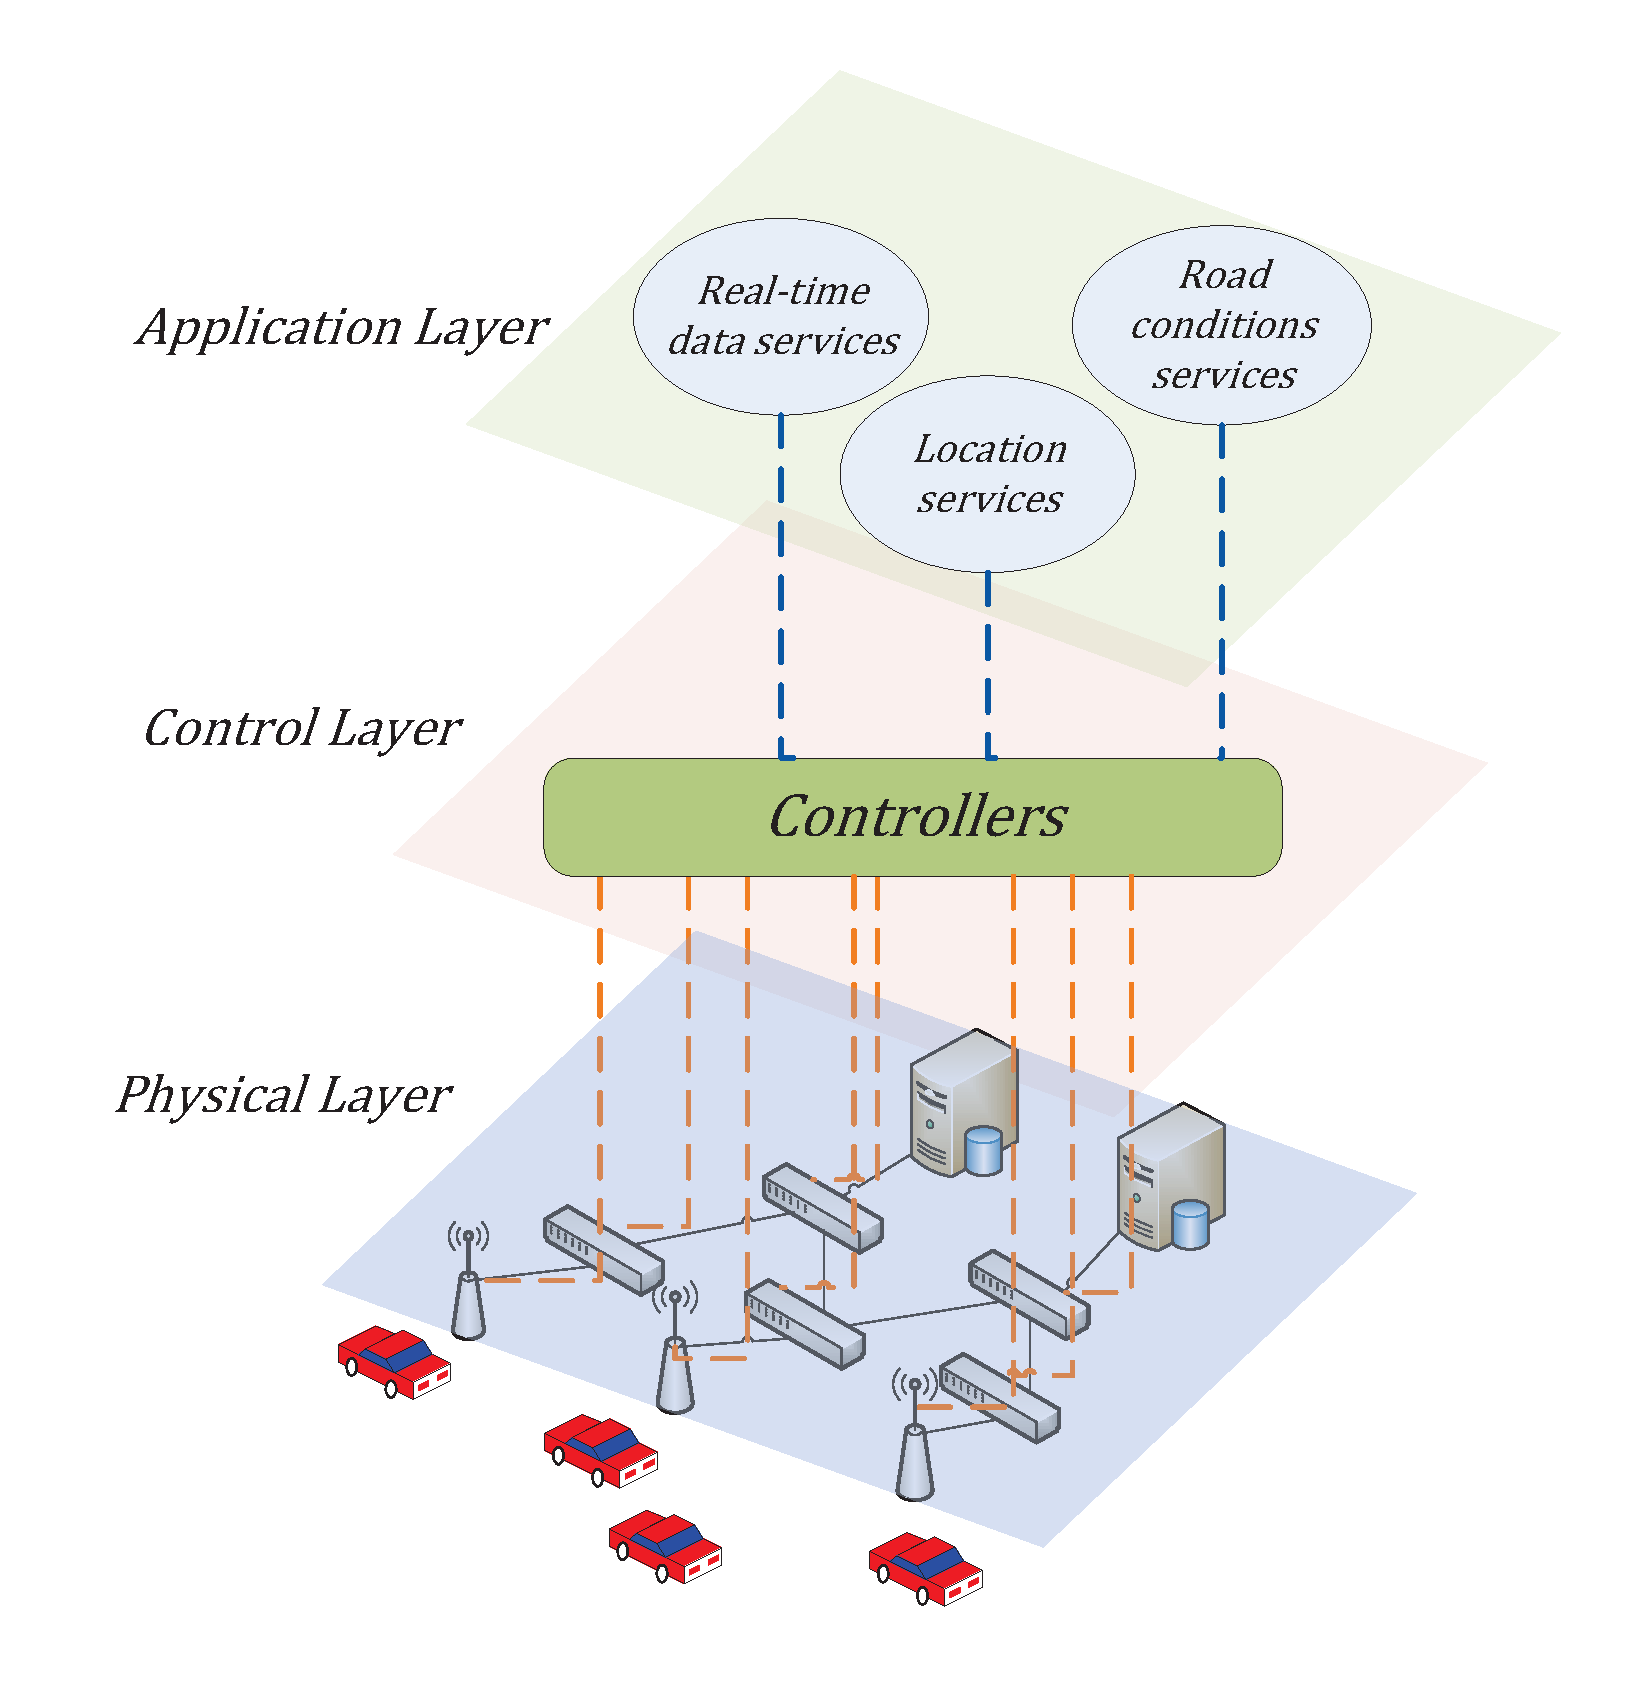
\includegraphics[width=0.9\columnwidth,height=2.5in]{figures/fig-2-24.eps}
% \vspace{-0.2in}
\caption{SDIV的三层架构模型。} \label{fig2}
\end{center}
% \vspace{-0.3in}
\end{figure}

\subsection{工作流程}



%After introducing the SDIV components, we describe how SDIV works with two scenarios as depicted in Fig. ~\ref{fig3}.


\begin{figure} [t]
\begin{center}
\begin{tabular}{c}
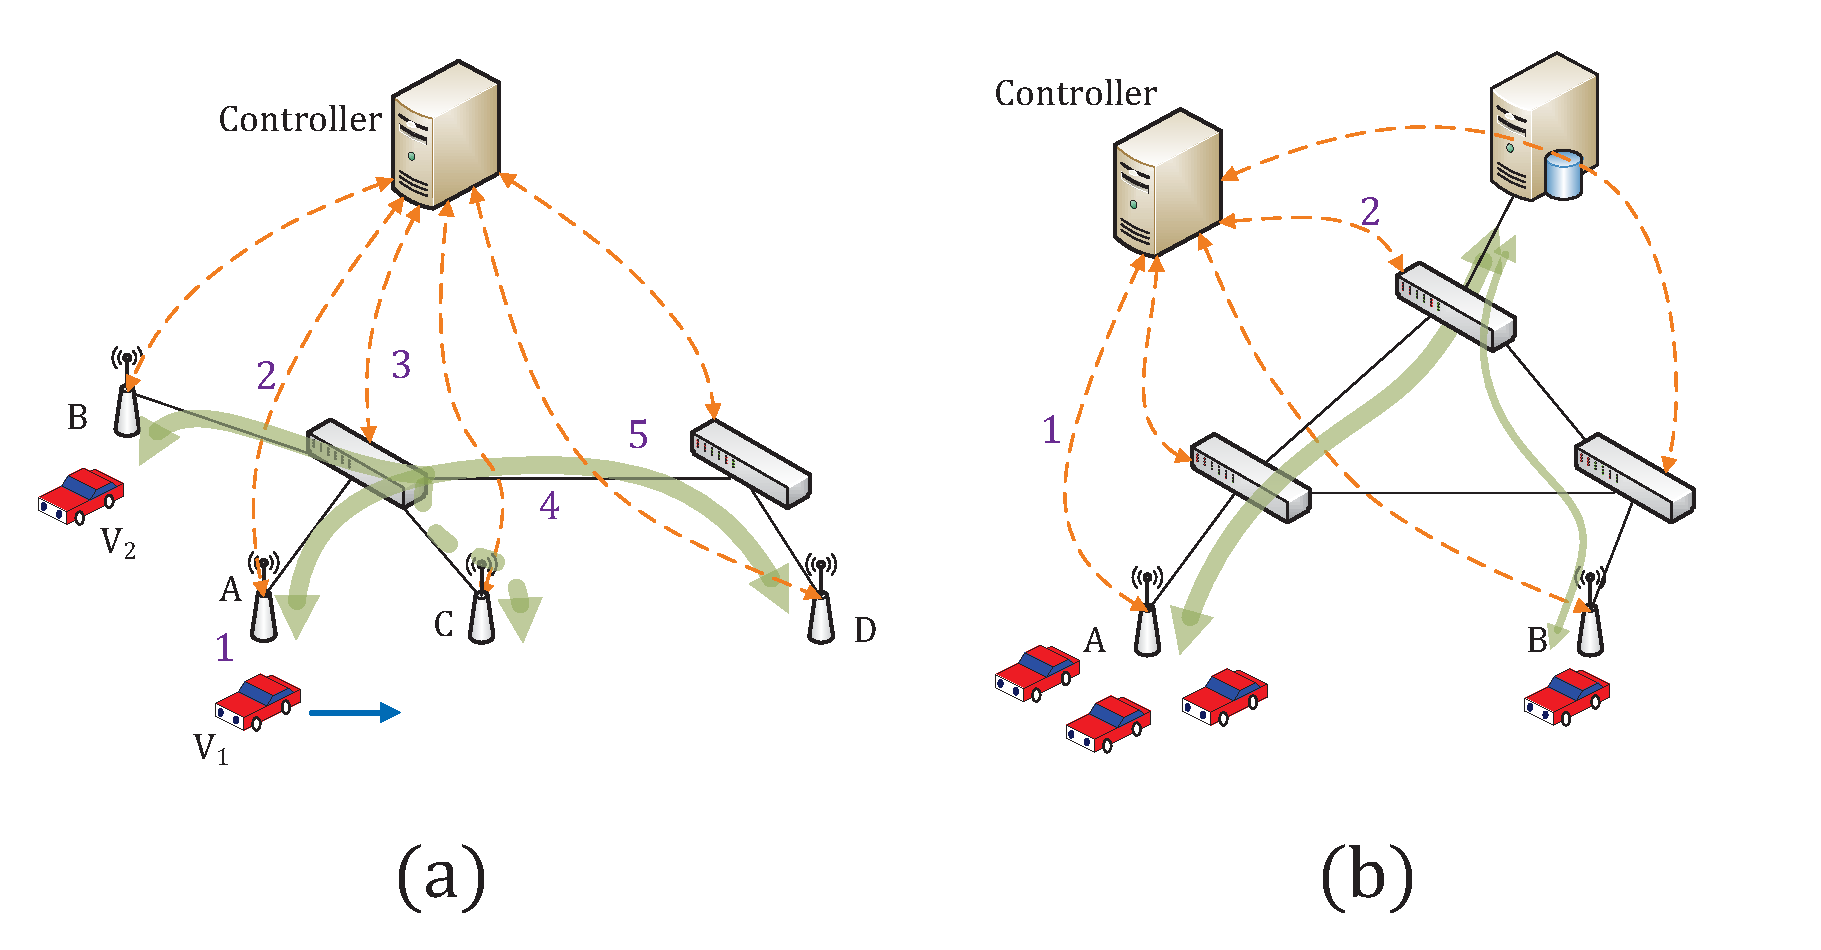
\includegraphics[width=1\columnwidth]{figures/fig-3-29.eps} \\
\end{tabular}
\caption{(a):通过分析车辆状况,控制器可以提前下发流规则(虚线)以降低额外请求;(b):控制器通过全局信息,实现智能带宽分配。} \label{fig3}
  \end{center}
  % \vspace{-0.3in}
\end{figure}

给出SDIV架构后,我们这里通过两个场景来描述SDIV的工作流程(如图~\ref{fig3})。
图~\ref{fig3}(a)描述的是一个车辆试图接受从路况摄像头发过来的路况信息的典型场景。

%Fig. ~\ref{fig3}(a) describes a typical scenario where a vehicle wants to receive the information about road conditions (maybe three blocks away from its current location) via surveillance cameras.

第一步,车辆$V_{1}$发送请求至附近的路旁AP;第二步,因为当前没有规则匹配该数据包,交换机(AP)$A$转发该数据包至控制器;第三步,控制器识别数据包头,并根据车辆的请求、车辆状况(例如,位置,速度、方向等)以及网络状况下发流规则;第四步,根据下发的规则,沿途的交换机转发数据包至目的节点$D$(即路况摄像头);第五步,从摄像头$D$传送过来的数据经过上述二至四的步骤最终到达车辆$V_{1}$。当车辆的数量增加时(即车辆$V_{2}$出现在了$B$附近),我们需要一个可拓展的方法去下发流规则,而非简单地重复上述步骤。同时,为了避免由于车辆移动性带来的数据传输中断,我们需要事先在$C$下发流规则。

%In Step 1, vehicle $V_{1}$ sends a request to a nearby road-side AP as shown in Fig.~\ref{fig3}(a); in Step 2, since there is no rule matching the header of the flow's first packet, the switch (AP $A$) encapsulates and forwards the packet to the controller; in Step 3, the controller recognizes the header and installs rules based on the vehicle's requests and information (e.g., location, speed and direction) and also the current network state; in Step 4, switches along the path towards the destination forward the matched packet to given ports based on the rules installed; in Step 5, the data flow from the surveillance camera ($D$) to the vehicle, goes through the same procedure as described in Steps 2-4. When the number of vehicles increases ($V_{2}$ at $B$ appears), there needs a scalable approach to installing rules for data transmission. The conditions (e.g., directions) of vehicles should be considered for installing rules, e.g., installing rules at $C$ in advance.

图~\ref{fig3}(b) 描述的是车辆通过附近AP与服务器进行连接并上传车辆信息,如速度和位置。在该数据上传场景中,控制器通过分析哪一个AP收到的数据包比较多,可以判断哪一个AP附近车辆较多,进而可以尽心更优化的资源调度。第一步,控制器分别从两个AP节点$A$和$B$收集数据包。当交换机收到数据包但没有相应匹配流规则时,则发送数据包至控制器。第二步,根据目的地址,控制器下发流规则到交换机中。此时,控制器可以发现$A$附近的车辆数量较多,因此可以分配更高的带宽给$A$。

%Fig.~\ref{fig3}(b) describes a scenario where vehicles need to build connections with the server through nearby APs for data uploading such as their current speed and location. The upper layer application (different from the servers in the network) can benefit from the data uploading scenario for analyzing road conditions. If the controller receives many packets from a particular AP, it can tell that there are many vehicles in this area compared with other places receiving few packets only. In Step 1, the controller gathers the information from APs $A$ and $B$. When switches receive packets with no rule matching, they send the packets to the controller. In Step 2, the controller installs rules in switches according to the destination addresses. If the upper layer application finds more vehicles in $A$ than in $B$, it can allocate more bandwidth to $A$.

除此之外,在考虑大规模的多播和车辆的移动性时,SDIV有着更大的优势。随着连接一个摄像头的车辆增多,可以想到用多播进行数据传输达到更高效的数据传输。虽然密集模式的多播在小规模网络有很好的效果,随着数据传输范围的变大,AP上不断增多的$(S,G)$项(S:源IP地址,G:组播IP地址)以及为了建立SPT(Shortest Path Tree)而周期性发送的广播消息限制了数据传输的进一步拓展。为了实现快速的嫁接,由于控制层和数据层的强耦合,$(S,G)$项需要被每一个路由器所保留(即使当前没有被该路由器使用)。如图~\ref{fig3}(a)所示,AP节点$B$也需要保留$(S,G)$项为了使新来的车辆$V_{2}$快速获取数据。车辆的移动性也给传统的网络技术带来了困难。如图~\ref{fig3}(a)所示,当车辆$V_{1}$从$A$来到$C$时,车辆需要重新发送请求从而导致数据接收的中断,同时也给$D$节点的摄像头带来了困难。在我们的设计中,我们通过预测车辆可能行驶的路径解决移动性问题。我们会在预测出的路径沿途的AP上实现下发实现多播的流规则。而沿着SPT的数据传输路径进行多播无法解决移动性问题,这是因为数据传输的最短路径不一定符合车辆行驶的路径。

%In addition, SDIV is more attractive when considering large-scale multicast and mobility of vehicles. As the number of vehicles connecting to one camera increases, it is easy to think of multicast for the efficiency of data transmission. Although dense-mode multicast (reasonable for cameras) goes well in small networks, as the range of data transmission increases, the growing number of $(S,G)$ \textcolor{blue}{(S: Source IP, G: Group IP)} entries kept in APs (or switches) and broadcasting messages periodically for establishing shortest path tree (SPT) limit the scalability of data transmission. The mixed model of control and data planes makes it necessary to keep $(S,G)$ entries even not used currently at every router for a fast graft. In Fig.~\ref{fig3}(a), it is necessary to reserve $(S,G)$ entries at AP $B$ for a new coming vehicle $V_{2}$. The mobility of vehicles also brings difficulty to traditional network technologies. Vehicle $V_{1}$ moving from $A$ to $C$ as described in Fig.~\ref{fig3}(a) needs to send another request for retrieving data, which results in interruption of data stream and extra workload of the surveillance camera ($D$). In our design, we address the mobility problem by predicting the most possible path that the vehicles would choose and set the rules in flow tables in advance to multicast the packets from nearby APs along the path. Multicast along the data transfer path in SPT cannot address the mobility issue since the shortest path for data transmission seldom matches the driving path.

以下表格总结了SDIV和传统网络技术(多播)的优劣势比较。相比传统多播方法需要周期性广播消息以搭建SPT,SDIV通过利用OpenFlow,即只有当数据包没有匹配流规则时才需要下发所需规则,实现了响应式的流规则下发方式,进而去除了周期性广播消息的需求。该响应式方式也让交换机可以保留最少数量的流规则,而非传统方式中的大量的$(S,G)$项。同时,基于全局的网络状态信息,控制器上的应用可以选择车辆可能行驶的路线并提前设置流规则进而实现数据传输的连续性。

%Table 1 summarizes the benefits of SDIV against traditional network technologies (multicast) besides its open interface of network equipment. Compared to the traditional multicast method that needs to broadcast messages periodically for establishing SPT, SDIV leverages the benefits of OpenFlow that makes switches forward packets with no matching rule in a flow table to the controller and then the controller installs rules for the packets. It is a reactive mode and rids the need to broadcast messages periodically. This reactive mode also makes it possible that the switches only need to keep the least number of rules in their flow tables instead of keeping $(S,G)$ entries at routers in a traditional multicast method. With the support of an up-to-date, global view of the network topology and traffic states, the application in the controller is able to compute the most possible path that a vehicle would choose and installs rules in advance for providing persistent connection between vehicles and devices.

\begin{table}[t]
 \centering
 \begin{tabular}{c|c}
  \hline
  传统网络技术(多播) & SDIV \\
  \hline
  \hline
  劣势: 周期性广播消息 & 优势: 响应式方式 \\
 \hline
 劣势: 路由器上保存$(S,G)$项& 优势: 当需要时设置 \\
 \hline
 劣势: SPT不符合车辆行驶路线 & 优势: 根据车辆状态预测行驶路线\\
  \hline
  优势: 不需要控制器 & 劣势: 需要控制器 \\
  \hline
 \end{tabular}
 \caption{\label{table1}传统网络技术与SDIV}
\end{table}

\section{优化的流规则下发}

在描述完SDIV的架构以及如何工作后,我们接下来会给出流规则下发问题的解决方案,并说明简单的下发流规则会导致的后果。

%Having described the SDIV architecture and how SDIV works, we give a solution for the rule installation problem and explain that it could bring significant complexity and overhead if naively installing rules are adopted for packet forwarding. We consider a real-time query service as the context to explain the necessity of its optimal solution.

在实时查询服务中,如果控制器简单地根据车辆的请求下发流规则,则由于Ternary Content-Addressable Memory (TCAM)有限的存储容量,流表的容量大小会成为系统性能的瓶颈。因此,我们需要建立一个紧凑的流表以放入更多的决策策略。对于每个数据流的建立,都需要两条流规则来分别处理发送请求和接受数据。即使我们只考虑第二个数据流,因为请求的数据流仅在开始时使用,并且可以通过OpenFlow交换机中的超时机制删除,我们仍然需要为每个流至少分配一个规则。似乎每个流使用一个规则对于流表来说足够紧凑,但实际上车辆会试图同时连接多个监控摄像头。因此,我们需要在每个交换机上对每个此类数据流设置规则,即使这些数据流都具有相同的目标。总而言之,我们需要减少转发到控制器的数据包数量并同时建立紧凑的流表。

%In a real-time query service, if the controller simply installs rules for the requests from drivers, the size of flow tables will incur the performance bottleneck due to the limited size of ternary content-addressable memory (TCAM) in switches. Thus, it is important to produce compact tables to fit more cached policy decisions in the switches. For each flow established, two rules are needed at the selected switches for sending the request packets and receiving the packets from the destination. Even if we only consider the second data flow, since the request flow is only useful at the beginning and can be deleted via timeout mechanism in OpenFlow switches, we still need at least one rule for each flow. It sounds that one rule for each flow is compact enough for a flow table, but in reality drivers attempt to connect multiple surveillance cameras at the same time. As a result, we need to install rules for every such data flow at every selected switch even though these flows all have the same destination. To summarize, we have to reduce the number of packets forwarded to the controller and establish a compact flow table due to the limited size of TCAM at switches.

图~\ref{fig4}描述了一个实时查询服务的基本工作流程。假设$V_{1}$想要获得道路(或十字路口)$E$的状况。这里,状况可以是视频或存储在路边设备中的任何其他种类的数据。第一步,$V_{1}$向AP节点$A$发送请求,然后数据流转发到$E$。在确认来自$V_{1}$的请求后,$E$将数据发送到AP节点$A$。最后,$A$将数据传输到$V_{1}$并完成数据传输。整个过程很简单,但可能会带来显着的性能损失。如图~\ref{fig4}所示,考虑另一车辆$V_{2}$想要获得$E$信息的情况。同时,考虑$V_{2}$在$V_{1}$的前方。当$V_{2}$重复与$V_{1}$相同的过程时,会建立另一条从$E$到$B$的路径,这使得交换机$D$对于相同的路径安装两条规则。结果,随着连接到$E$的车辆数量的增加,沿途的交换机的流表大小可能达到最大值,从而降低了实时查询服务的性能。此外,当$V_{1}$移动到另一个地方时,它也需要再次发送请求。

%Fig.~\ref{fig4} depicts the basic scenario that how a real-time query service works. Suppose that $V_{1}$ wants to obtain the conditions of road (or crossroads) $E$. Here, the conditions can be a video or any other kinds of data stored in the roadside devices. At the first step, $V_{1}$ sends a request to AP $A$ and then the data flow is forwarded to $E$. After confirming the request from $V_{1}$, $E$ sends data to AP $A$. Finally, AP $A$ transmits the data to $V_{1}$ and completes the data transmission. The entire process is simple, but the simplicity may introduce significant performance penalty. As shown in Fig. ~\ref{fig4}, consider the situation that there is another vehicle $V_{2}$ that wants to get the information of $E$. And also the $V_{2}$ is ahead of $V_{1}$. When $V_{2}$ follows the same procedure as $V_{1}$ does, there is another path from $E$ to $B$ established, which makes switch $D$ install two rules following the same path. As the result, as the number of vehicles connecting to $E$ increases, the flow table size at switches along the path may reach the maximum that in turn reduces the performance of the real-time query service. Moreover, when $V_{1}$ moves to another place, it needs to send a request again.

接下来,我们考虑另一个场景来说明优化的流规则下发的重要性。 $V_{1}$想要同时从$E$和$F$获取数据。交换机$B$和$D$需要设置更多规则以使数据流传输到$A$,即使两个流($E \to A$和$F \to A$)具有相同的目的地。如果$V_{3}$请求相同的服务,这种情况会变得更加复杂。为了使$C$下面的$V_{3}$接收数据,需要构建一条新路径(即,相同的数据流将在三辆车辆所连接的交换机处分开,因而该交换机成为分支节点),这再次增加了流表的大小。车辆的移动性也增加了复杂性并降低了实时查询服务的性能。

%Next, we consider another example to show the importance of optimal rule installation. $V_{1}$ wants to get the data from $E$ and $F$ at the same time. Switches $B$ and $D$ need to install more rules to make data flow transmitted to $A$, even though both flows ($E \to A$ and $F \to A$) have the same destination. Such situations become more complex if $V_{3}$ requests the same service. To enable $V_{3}$ at $C$ to receive data, there is a need of building a new path (i.e., the same data flow will split at the attaching switch of the three vehicles, then the switch becomes a branching node), which again increases the flow table size. The mobility of vehicles increases the complexity and degrades performance of the real-time query service as well.

为了解决规则下发问题并减缓流表大小的增长,我们考虑将无线数据平面(用于车辆和AP之间的通信)与有线数据平面(用于交换机之间的通信)分开,并提出目的地驱动模型用于有线数据平面。当车辆从附近的AP接收数据时,它们不关心数据如何在有线数据平面中传输。相反,它们只想要一个持久的连接,即使它们的位置随着时间而变化。为了有效地进行分离,我们引入了三种技术:1. 使用多播地址作为摄像头到车辆的最后一跳地址;2. 根据车辆的状况预先在最可能的路径中安装规则; 3. 当数据包到达分支节点时修改数据包头。

%To solve the rule installation problem and mitigate the flow table size growth, we propose to separate the wireless data plane (for communication between vehicles and APs) from the wired data plane (for communication among switches) and develop a destination-driven model (given later in Section ~\ref{Modify address}) for the wired data plane. When vehicles receive data from nearby APs, they do not care how data transmitted in the wired data plane. Instead, they just want a persistent connection even their locations change over time. To make the separation efficiently, we introduce three techniques: (1) using a multicast address as the last hop address from cameras to vehicles, (2) installing rules in the most possible path in advance according to the conditions of vehicles, and (3) modifying the headers when packets come to branching nodes to be defined.


%%\begin{figure} [t]
%%\begin{center}
%%\includegraphics[width=0.7\columnwidth]{fig5-modified-type-large.eps}
%%
%%\caption{有线数据平面和无线数据平面的分离。虚线表示数据流可以增量式的建立。
%%A separation between wired data plane and wireless data plane. Dash line means that data flow may be established incrementally from a existing one.} \label{fig5}
%%\end{center}
%%\end{figure}




\subsection{使用多播地址作为最后一跳} \label{Multicast address}

我们利用多播地址来解决移动性问题并增强SDIV的可扩展性。每个监控摄像头都有一个唯一的组播地址,可以通过传统网络中的相同方法从MAC地址生成。多播地址可以在从摄像头到车辆的最后一跳中用于无线数据平面中的数据传输。车辆$V_{1}$接收目的地址为$E$多播地址的数据包,如图~\ref{fig4}所示。使用多播地址的优点是显而易见的,即在已配备规则的AP范围内的每个车辆可以在不发送新请求的情况下获得实时数据。此外,在实时查询服务中,必须将第一个用户请求包转发到控制器以安装规则。如果每个请求都需要联系控制器进行规则安装,则会导致控制器成为严重的瓶颈。多播地址可以有效地解决这个问题。在第一辆车通过控制器的参与并连接摄像头后,数据流开始进行多播传输(沿着到达目的地的路径),并且对同一摄像头请求的每辆新车都会直接接收数据而不用发送请求,这降低了联系控制器的频率。例如,在图~\ref{fig4}中,如果有另一车辆想要查看$E$的状况,它可以在$V_{1}$发送请求后不用发送请求而直接接收数据。

%We utilize multicast addresses for the purpose to deal with the mobility and enhance the scalability of SDIV. Every surveillance camera has a unique multicast address which can be generated from a MAC address by the same method in traditional networks. Multicast addresses can be used in the last hop from cameras to vehicles for data transmission in the wireless data plane. Vehicle $V_{1}$ receives packets with the destination address of $E$'s multicast address in Fig.~\ref{fig4}. The advantage of using multicast addresses is apparent, i.e., every vehicle, within the range of an AP that has been equipped with the rule, can get the real-time data without sending new requests. Furthermore, in a real-time query service, the first packet of user requests has to be forwarded to the controller for installing rules. If every request needs to contact the controller for rule installation, it leads to a serious bottleneck at the controller since both computational capacity and bandwidth are limited. A multicast address can address this problem efficiently. After the first vehicle connected the camera with the intervention of the controller, the data flow starts to multicasts (along the path to the destination), and every new vehicle asking for the same camera receives the data without sending the request, which reduces the frequency of contacting the controller. For example in Fig.~\ref{fig4}, if there is another vehicle that wants to see the conditions of $E$, it can receive the data without sending a request after $V_{1}$ sent the request.

由于OpenFlow交换机中TCAM的大小有限,我们需要从流表中删除无用的规则。在我们的设计中,我们使用OpenFlow中的超时机制来删除规则。对于每一流规则,交换机都会维护一个变量,该变量表示是否在一段时间$T$秒内,没有数据包到达匹配该流规则。实际上,OpenFlow中,通过向流表条目添加``空闲时间"值来实现超时机制。与相等的超时时间相比,我们根据离目的地的距离在交换机中选择不同的超时值。现实情况中,随着离目的地越近,对目的地感兴趣的车辆数量会越大。因此我们在离目的地更近的交换机设置更大的超时值。例如图~\ref{fig4}所示,超时值$T_{i}$ 在交换机$i$符合约束条件:$ T_{A} < T_{B} < T_{D} < T_{E}$。离信息源越近,数据流的变化越小因为这些流会合并成稳定的数据流。而稳定的数据流需要比不稳定数据流具有更长的超时。

%Due to the limited size of TCAM in OpenFlow-supported switches, we need to remove the useless rules from flow tables. In our design, we use timeout in OpenFlow to delete rules for saving flow table resources. A switch maintains a per-flow-entry variable that indicates if there has ever been a period of $T$ seconds in which no packet arrived for the flow. In practice, in OpenFlow, this is maintained by adding an ``idle timeout" value to a flow entry. Instead of setting equal values of timeout, we choose different values of timeout in switches depending on the distance away from the destination. In reality, the number of vehicles interested in the destination gets larger as they are closer to the destination. Then we set larger values in timeout for the closer switches to the destination. As an example in Fig. ~\ref{fig4}, the timeout value $T_{i}$ in switch $i$ meets the constraint: $T_{A} < T_{B} < T_{D} < T_{E}$. The closer to the information source, the less changes on data flows, since these flows would merge to a stable singe flow. The stable data flow would require a long timeout than unstable flows.


\begin{figure} [t]
\begin{center}
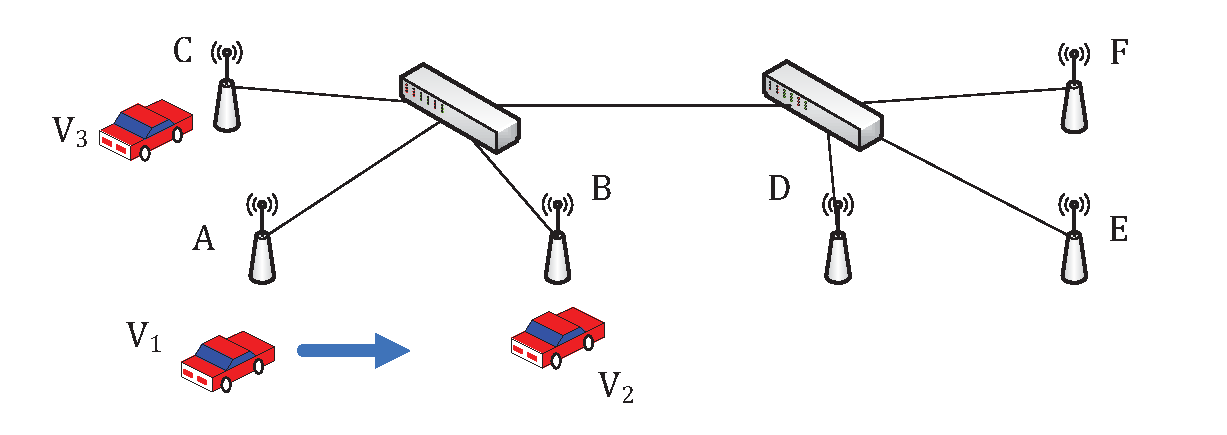
\includegraphics[width=1\columnwidth]{figures/fig-4-31.eps}

\caption{$V_{1}$ 同时连接$E$和$F$。$V_{2}$在$V_{1}$到$E$的路径上并向$E$请求数据。$V_{3}$也同时向$E$请求数据但在不同路径。} \label{fig4}
\end{center}
%\vspace{-0.3in}
\end{figure}

\subsection{路线预测并提前下发流规则} \label{Predict the path}

\begin{algorithm}[t]
\caption{PathFind($s,d,v$)}
\label{Algorithm 2}
\begin{algorithmic}[1]
%\algsetup{linenosize=\footnotesize}
%\footnotesize

\STATE{Algorithm PathFind($s,d,v$)}
\STATE{~~put $s$ into set $N$, $R$;}
\STATE{~~for each child node $c$ of $s$}
\STATE{~~~~if the angle between $v$ and $A(s,c)$ is less than 90 degree then}
\STATE{~~~~~~put $c$ into set $O$;}
\STATE{~~Find($s,O,d$);}
\STATE{~~return $R$;}
\STATE{Procedure Find($p,O,d$)}
\STATE{~~put $p$ into set $N$;}
\STATE{~~for each $n$ in $O$}
\STATE{~~~~if $n$ is $d$ then}
\STATE{~~~~~~put $n$ into set $R$;}
\STATE{~~~~~~finish;}
\STATE{~~~~put $n$ into set $N$;}
\STATE{~~~~remove $n$ from set $O$;}
\STATE{~~~~calculate $D(n,d)$, $D(p,n)$;}
\STATE{~~~~if $D(p,n)+D(n,d)<max$ then}
\STATE{~~~~~~$max = D(p,n)+D(n,d)$;}
\STATE{~~~~~~$r = n$;}
\STATE{~~put $r$ into set $R$;}
\STATE{~~for each child node $c$ of $r$}
\STATE{~~~~if $c$ not in set $N$ then}
\STATE{~~~~~~put $c$ into set $O$;}
\STATE{~~Find($r,O,d$);}
\STATE{~~return;}
\end{algorithmic}
% \vspace{-0.06in}
\end{algorithm}

为了处理SDIV中车辆的移动性,有必要预测车辆选择的最可能路线,然后沿路线预先安装规则,以便在车辆移动时保持数据传输不中断。预测这种路线的一种简单方法是计算最短路径,但实际上并不总是正确。我们设计算法$PathFind(s,d,v)$(算法\ref{Predict the path}),来找到拓扑中最可能的路径。这里$s$代表当前位置,$d$表示目的地,$v$表示车辆的方向。$ A(s,c)$表示$s$和$c$的角度,$D(n,d)$表示$n$和$d$之间的欧几里德距离。


%To deal with the mobility of vehicles in SDIV, it is necessary to predict the most possible path that a driver chooses and then install rules in advance along the path in order to keep data transmission uninterrupted while the vehicle is moving. A simple method to predict such a path is computing the shortest path, but it is not always a correct path in reality. We propose and describe $PathFind(s,d,v)$, in Algorithm 1 that finds the most likely path in a topology. Here $s$ is the current location, $d$ is the destination and $v$ is the direction of the vehicle. $A(s,c)$ denotes the angle of $s$ and $c$, $D(n,d)$ means Euclidean distance between $n$ and $d$. Note that Manhattan distance may also be used to cope with an urban environment.

作为准备工作(第三至五行),$PathFind$根据车辆的状况(例如,方向)过滤并得到的路径的可能的第一节点,这是因为车辆很少在街道中掉头。如图所示在十七至二十行,我们通过选择具有$D(p,n)+D(n,d)$最小值(即所选位置和目的地之间的距离)的节点来递归地应用$Find$来计算结果路径。最后,$Find$将目标标识为下一个节点并返回结果(第十二至十四行)。

%As the preparatory work (Lines 3-5), $PathFind$ filters the possible first node of a resulting path according to the condition (e.g., direction) of the vehicle, since the driver seldom turns back in a street. We apply $Find$ recursively to calculate the resulting path by choosing the node that has the minimum value of $D(p,n)+D(n,d)$, e.g., the distance between the chosen location and the destination as shown in Lines 17-20. In the current design, $D(n,d)$ denotes Euclidean distance between $n$ and $d$, but we can change it to a more intelligent calculation. Finally, $Find$ identifies the destination as the next node and returns the result (Lines 12-14).

我们在图~\ref{fig5}中应用$PathFind$。考虑一个位于$A$的车辆计划找到$F$的路线。首先,它根据当前位置的车辆方向设置$B$为$O$的值。然后发现$D$与$C$相比有更短的路径到$F$。因此,它选择$D$重新开始,发现$D$
直接连接到$F$并完成。结果$ A \to B \to D \to F $比最短路径$ A \to E \to F $更合理,因为实际上很少看到倒车行为。虽然路径$ A \to B \to D \to F $的时延比路径$ A \to E \to F $长,但是当车辆发现没有收到数据时,会发出更多请求。在这种情况下,车辆可能选择$B$作为其下一个位置,因此得到的路径优于最短路径,因为车辆可以在不发送另一个请求的情况下接收数据。在图~\ref{fig5}中,在预测路线上的交换机上安装规则($ A \to B \to D \to E $)后,多播地址也会使$V_{2}$直接接收数据而不用发送一个新的要求。
%
%We apply $PathFind$ in Fig.~\ref{fig5}. Consider a vehicle in location $A$ plans to find a path to $F$. First, it puts $B$ into set $O$ according to the direction of the vehicle at the current location. It then finds $D$ has a shorter path to $F$ compared with $C$. It chooses $D$ to start again, and finds $D$ that directly connects to $F$ and finishes. The result $A \to B \to D \to F$ is more reasonable than the shortest path $A \to E \to F$ since reversing a vehicle is rarely seen in reality (unless the distance difference is quite large). Though the delay of path $A \to B \to D \to F$ is prolonged comparing to path $A \to E \to F$, the vehicle sends more requests when it finds no data from its nearby AP. In this case, the vehicle more likely chooses $B$ as its next location, and thus the resulting path is better than the shortest path since the vehicle can receive data without sending another request. In Fig. ~\ref{fig5}, after installing rules at the switches along the predicted path ($A \to B \to D \to E$), the multicast address also makes $V_{2}$ receive data without sending a new request.
%



\subsection{分支节点修改数据包地址} \label{Modify address}

\begin{algorithm}[t]
\caption{ModifyAddress($s,d,path$)}
\label{Algorithm3}
\begin{algorithmic}[1]
%\algsetup{linenosize=\footnotesize}
%\footnotesize

\STATE{Algorithm ModifyAddress($s,d,path$)}
\STATE{~~for each node $n$ in $path$ do}
\STATE{~~~~$nx$ = the next node of $n$;}
\STATE{~~~~$setRule$ = false;}
\STATE{~~~~for each rule $r$ in $n$ do}
\STATE{~~~~~~$no$ = the node connecting the output port of $r$;}
\STATE{~~~~~~if $r$ matching $s$ and $no$ != $nx$ then}
\STATE{~~~~~~~~$act$ = forward to $nx$ and modify the destination address to $d$;}
\STATE{~~~~~~~~$emitRule(matchFor(d),act)$;}
\STATE{~~~~~~~~$setRule$ = true;}
\STATE{~~~~~~else if $r$ matching $s$ and $no$ = $nx$ then}
\STATE{~~~~~~~~$setRule$ = true;}
\STATE{~~~~if $setRule$ == false then}
\STATE{~~~~~~$act$ = forward to $nx$;}
\STATE{~~~~~~$emitRule(matchFor(d),act)$;}
\STATE{~~return;}
\end{algorithmic}
% \vspace{-0.06in}
\end{algorithm}

% \vspace{-0.05in}

\begin{figure} [t]
\begin{center}
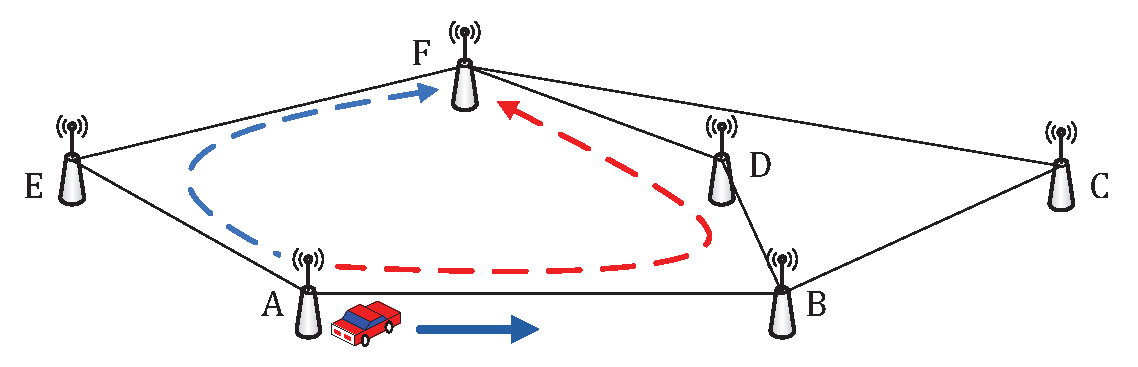
\includegraphics[width=0.9\columnwidth]{figures/fig-5-31.eps}
\caption{蓝色虚线代表当前位置到目的位置的最短路径。红色虚线代表车辆可能选择的路径。} \label{fig5}
\end{center}
% \vspace{-0.3in}
\end{figure}

在本小节中,我们将展示如何在交换机上安装规则。如算法~\ref{Algorithm3}所示,其主要思想是我们通过利用OpenFlow特性在分支节点(第八至九行)添加数据包头修改操作。输入$s$表示数据源,$d$表示车辆的当前位置,$path$由$PathFind$计算生成。当数据包匹配规则并修改匹配字段时,它将在转发到特定端口之前应用修改。修改后的地址使数据包转发到直接连接到车辆的交换机。通过使用地址修改算法,我们让具有不同源地址但相同目的地地址的数据包匹配相同的规则,从而减少规则数量并减少流表大小。我们将此方法称为目标驱动模型,因为它只需要匹配目标地址。

%In this subsection, we will show how to install rules at switches. The main idea is that we add a packet header modifying action at the branching nodes (Line 8-9) by leveraging the properties of OpenFlow as shown in Algorithm 2. The input $s$ denotes the source of data, $d$ denotes the current location of the vehicle and $path$ is computed by $PathFind$. \textcolor{blue}{When a packet matches a rule to modify the match field, it will first apply the modification before forwarding to a particular port, and this process is guaranteed by the OpenFlow protocol. The modified address makes the packet forwarded to the switch directly connecting to the vehicle.} We clarify that the rule matching $s$ means that the controller records the source address of every request, not the rule in the switch matches $s$. By using the address modification algorithm, we let packets with different source addresses but the same destination address match the same rule and hence reduce the number of rules and reduce the flow table size. We call this approach a destination-driven model, since it needs to match the destination address only.

如图~\ref{fig6}所示,数据流$F_{1}$和$F_{2}$均来自监控摄像头$S_{1}$,而$F_{3}$来自$S_{2}$。$F_{1}$由$V_{1}$请求。$F_{2}$和$F_{3}$的目标是$V_{2}$。假设$V_{1}$的当前位置是$C$,$V_{2}$的位置是$D$。在单播情况,$F_{1}$和$F_{2}$需要至少两个规则在交换机$A$和$B$;在多播情况下,$F_{2}$和$F_{3}$也需要至少两条规则在交换机$A$和$B$。然而这是低效的,因为$F_{1}$和$F_{2}$来自同一节点,而$F_{2}$和$F_{3}$具有相同的目的地。我们在交换机$B$(作为分支节点)上修改$F_{1}$和$F_{2}$数据包头中的目标地址。通过设置$F_{1}$和$F_{2}$的目标地址(即$F_{1} \to C$,$F_{2} \to D$),减少了交换机中的规则数量并可以提供更多服务。再假设$V_{2}$在开始时向$S_{1}$发送请求。每个交换机只需要一个规则来转发$F_{2}$。而当$V_{2}$从$S_{2}$获取数据时,交换机的规则仍适用。最后,当$V_{1}$需要来自$S_{1}$的数据时,它只需在交换机$B$上额外增加一个规则并匹配$(S_ {1},D)$以及一个修改操作。这里我们使用两个参数来表示包头,即(源地址,目的地址),以及流表中的匹配条件。该目标驱动模式将目标地址设置为流表中的匹配条件,合并同一目标的数据流的流规则,以减小交换机中流表的大小。在图~\ref{fig4}中,当$V_ {3}$加入时,它需要在分支交换机处进行地址修改以优化规则安装。

%
%As an example shown in Fig.~\ref{fig6}, data flows $F_{1}$ and $F_{2}$ are both generated from surveillance camera $S_{1}$, and $F_{3}$ comes from $S_{2}$. $F_{1}$ is requested from $V_{1}$. $F_{2}$ and $F_{3}$ are destined to $V_{2}$. Suppose that $V_{1}$'s current location is $C$ and $V_{2}$ is at $D$, $F_{1}$ and $F_{2}$ need at least two rules at switches $A$ and $B$ in unicast, and $F_{2}$ and $F_{3}$ need two rules at least at switches $A$ and $B$ in multicast. This is not efficient since $F_{1}$ and $F_{2}$ come from the same node, and $F_{2}$ and $F_{3}$ have the same destination. We modify the destination address in the header of packets in switch $B$ (as a branching node) for $F_{1}$ and $F_{2}$. By setting the destination address of packets in $F_{1}$ and $F_{2}$ ($F_{1} \to C$ and $F_{2} \to D$), the number of rules in switches is reduced and so is the size of the flow table for more services. Let's assume $V_{2}$ sends a request to $S_{1}$ in the beginning. Each switch only needs one rule to carry $F_{2}$. When $V_{2}$ asks data from $S_{2}$, the rules at switches still suit. Finally, when $V_{1}$ requires data from $S_{1}$, it just increases one rule at switch $B$ via matching $(S_{1}, D)$ with an action of modification. Here we use two parameters to represent the packet header, namely $(source address, destination address)$, and so are the match conditions in the flow table. This destination-driven mode emphasizes the destination address as matching conditions in the flow table, and generalizes the data flow demands of the same destination for reducing the size of flow tables in switches. In Fig.~\ref{fig4}, when $V_{3}$ joins, it needs address modification at the branching switch to optimize rule installation.

接下来,我们通过两种情况来分析优化的规则下发:1. 一台服务器连接多台车辆;2. 一台车辆连接多台服务器。对于第一种情况,传统的规则安装仅根据源地址将数据包转发到给定端口,而在路径的每个交换机上需要一个规则。在我们提出的规则下发方法中,我们在每个交换机上需要一个规则用于转发,并且需要在分支节点处修改数据头的操作。由于修改地址操作可以与OpenFlow中的转发操作组合作为一个规则操作,因此与传统规则下相比,规则的数量不会改变。对于第二种情况,我们假设有一辆车辆($v$)连接到多个服务器($s_1,s_2, ... s_n$),并且我们规定$s_i$离$v$的距离为$h_i$(跳数)。设$ L_i $表示用于$ v $和$ s_i $之间数据传输的一组链路。因此,我们有$|L_i| = h_i$。因此传统方法需要$\sum_{i=1}^{n} h_i$条规则,而通过我们优化的规则安装,我们需要$|L|$条规则,其中$L = \bigcup{(L_{1}, L_{2}, ... L_{n})}$。考虑一个极端情况,任何两组链路$L_i$和$L_j$都没有共享链路,则我们有$|L| = \sum_{i=1}^{n} h_i$。在这种情况下,我们提出的方法所需的规则数量与传统方法相同。对于其他大多数场景,$|L| < \sum_{i=1}^{n} h_i$,这意味着我们提出的方法减少了规则的数量。总而言之,我们优化的规则的最坏情况包括上述第一种情况和第二种的极端情况不会改变规则的数量,而最好的情况可以在一辆车连接到多个服务器时减少很多规则。

%
%Next, we give an analysis of improved rule installation for two cases: (a) one server connects to multiple vehicles and (b) one vehicle connects to multiple servers. For the first one, the traditional rule installation that forwards packets to given ports simply based on the source address needs one rule at each switch along the data path. In our proposed rule installation method, we need one rule at each switch for forwarding and an extra action for modifying data header at the branch nodes. Since the modifying address action can be combined with the forwarding action in OpenFlow as a set of actions of rule, the number of rules does not change compared with the traditional rule installation. For the second one, we assume that there is one vehicle ($v$) connecting to multiple servers ($s_1, s_2,...s_n$), and $s_i$ is $h_i$ hops away from $v$. Let $L_i$ denote a set of links used for the data flow between $v$ and $s_i$. Hence, we have $|L_i| = h_i$. Then the traditional approach needs $\sum_{i=1}^{n} h_i$ rules, while by our improved rule installation, we need $|L|$ rules where $L = \bigcup{(L_{1}, L_{2}, ... L_{n})}$. Considering one extreme scenario that any two $L_i$ and $L_j$ have no sharing link. Then we have $|L| = \sum_{i=1}^{n} h_i$. In this scenario, the number of rules needed by the proposed approach is the same as the traditional method. For many other scenarios, $|L| < \sum_{i=1}^{n} h_i$, which means that the use of the proposed one reduces the number of rules. In summary, the worst case of our improved rule installation including the case one and the extreme scenario of case two does not change the number of rules while the best case could reduce many rules when there is one vehicle connecting to multiple servers.
%



\begin{figure} [t]
\begin{center}
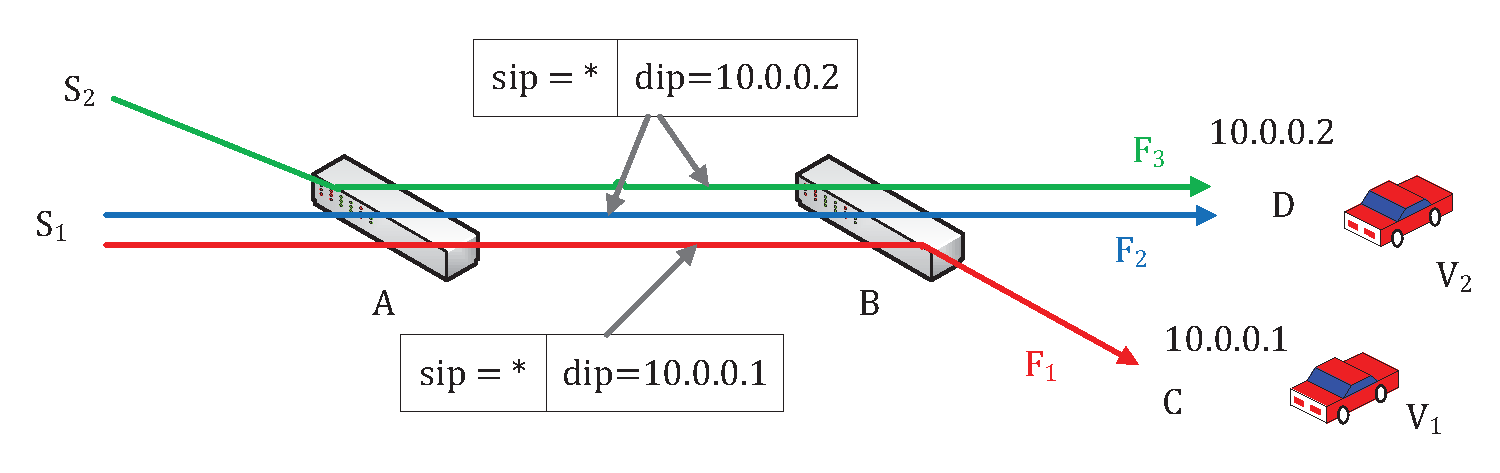
\includegraphics[width=1\columnwidth]{figures/fig-6-31.eps}
\caption{数据流$F_{1}$(红色)从$S_{1}$到$C$;数据流$F_{2}$(蓝色)从$S_{1}$到$D$;数据流$F_{3}$(绿色)从$S_{2}$到$D$.匹配条件只依赖于目的地址。} \label{fig6}
\end{center}
% \vspace{-0.3in}
\end{figure}



\begin{figure} [t]
\begin{center}
\begin{tabular}{cc}
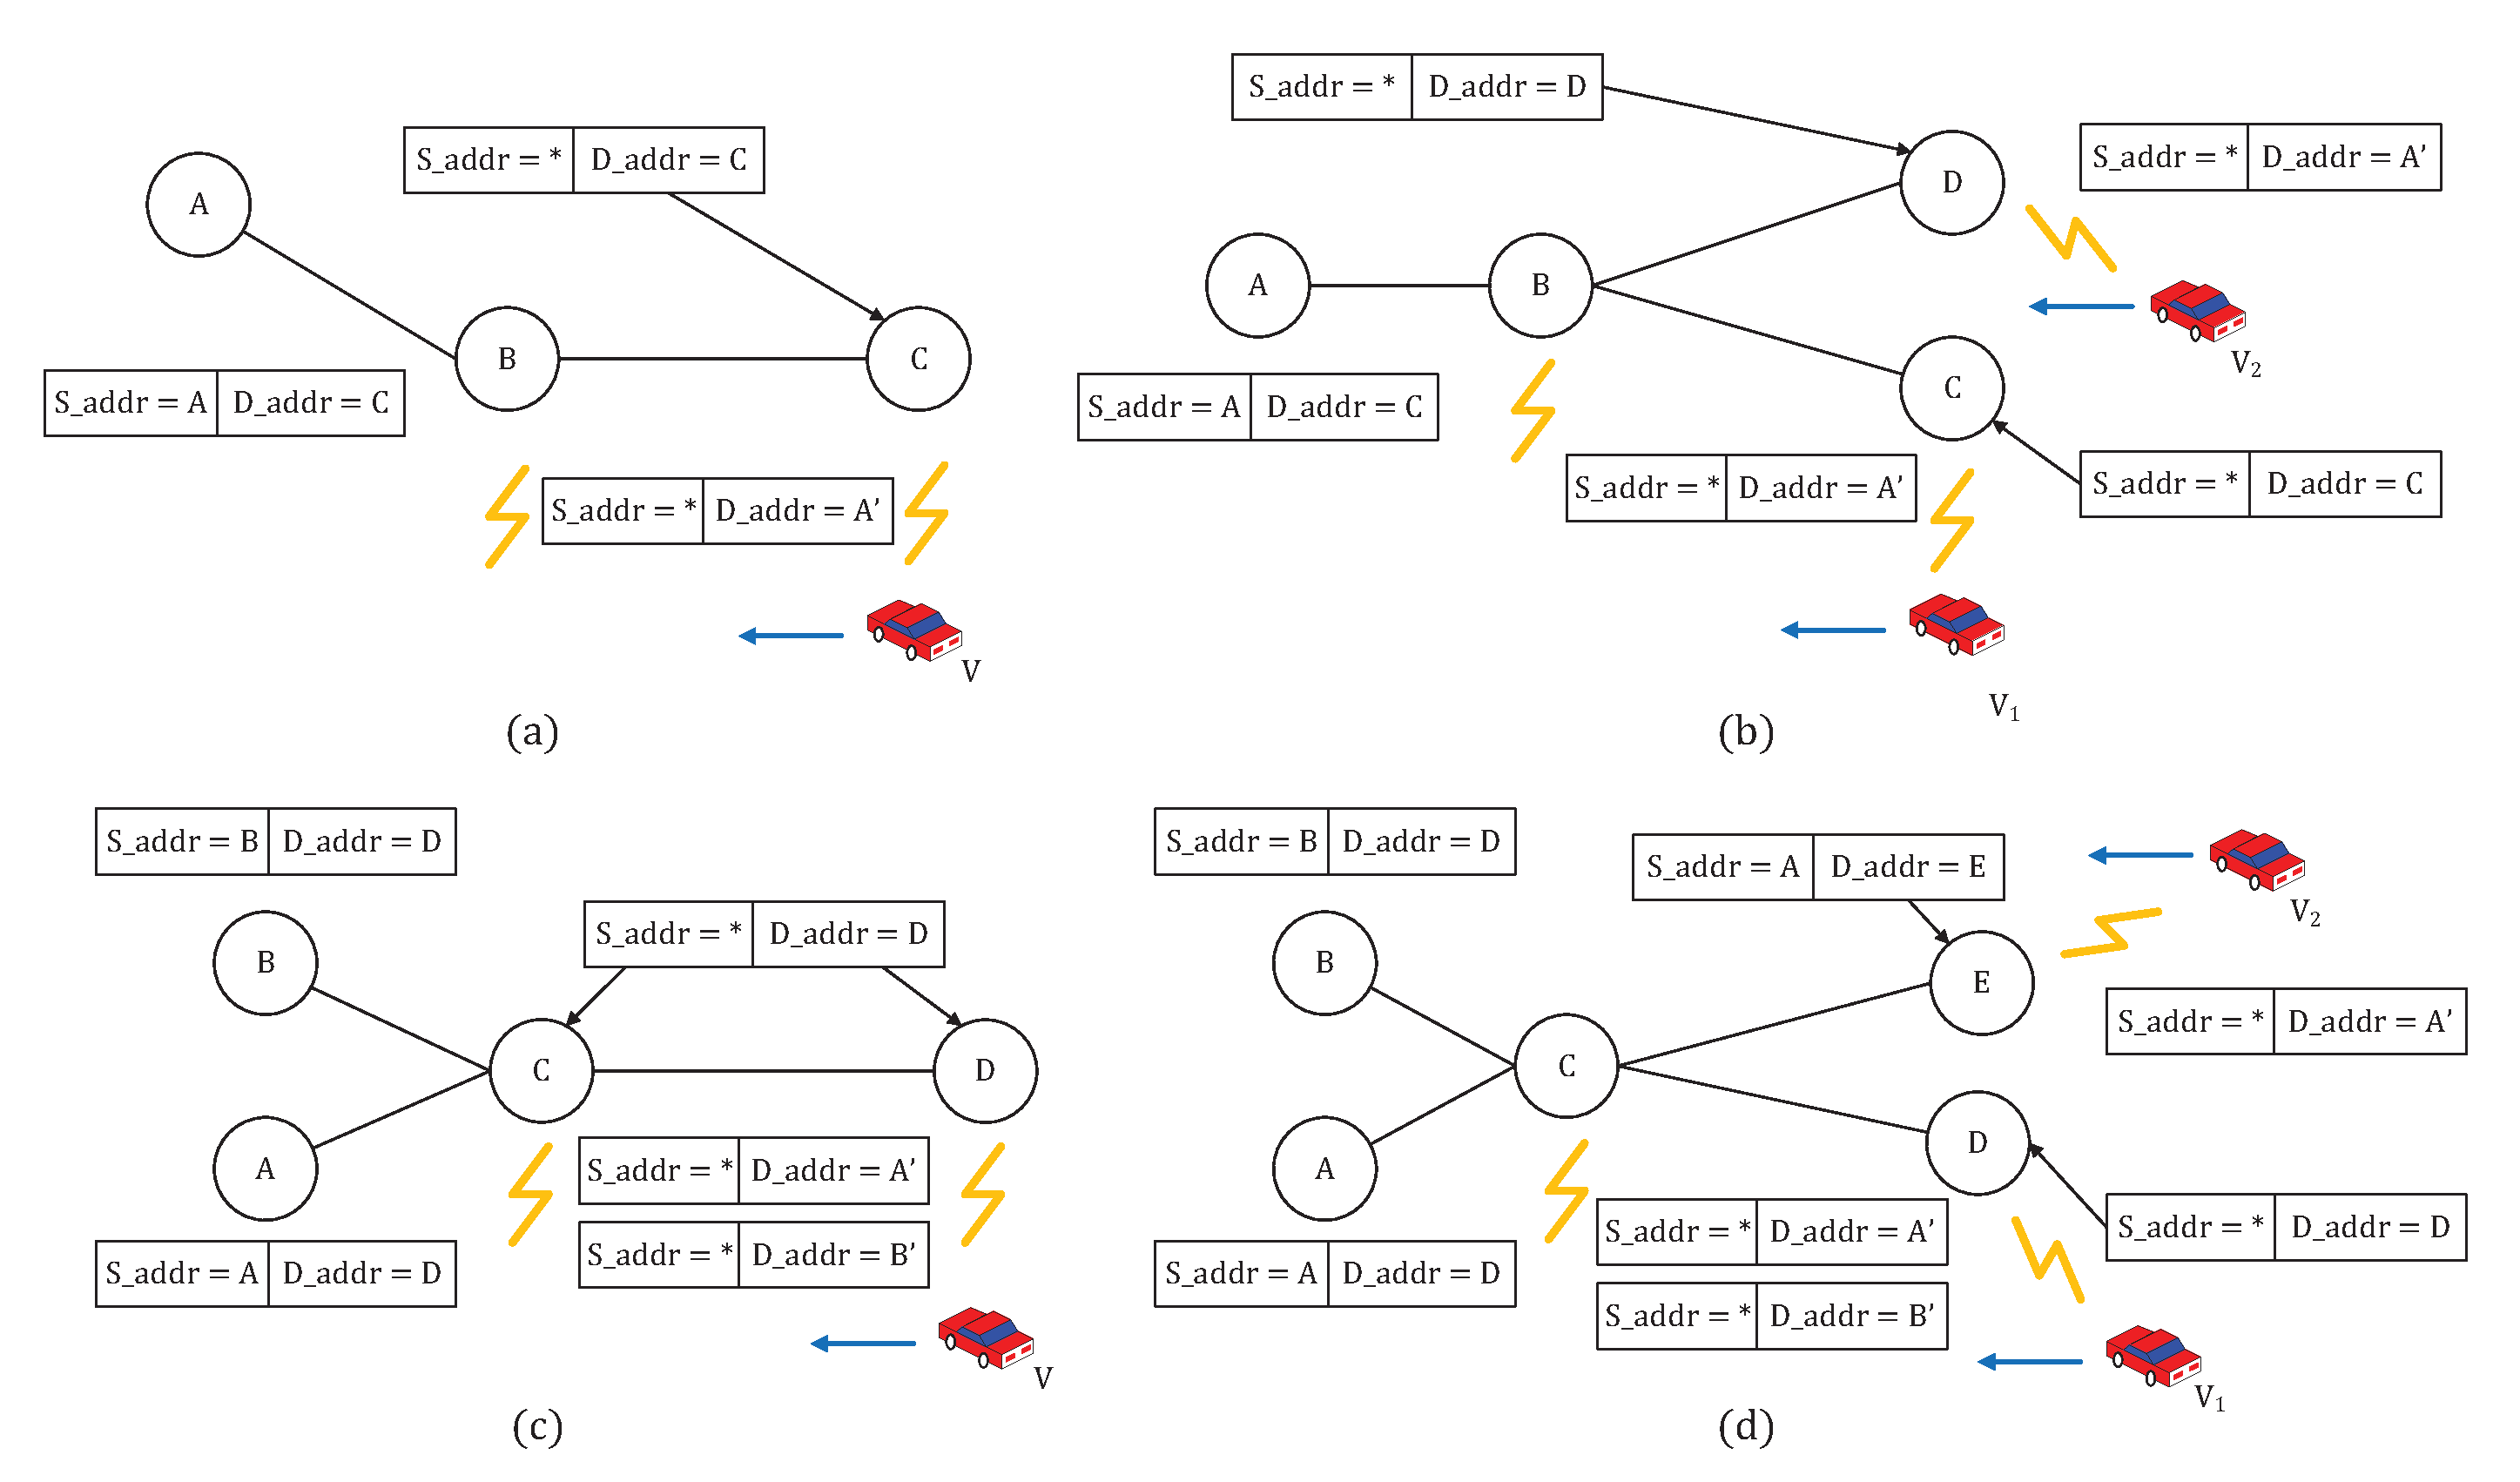
\includegraphics[width=\columnwidth]{figures/fig8-big.eps}
\end{tabular}
\caption{(a):1对1场景即$V$接受$A$的数据;(b):N对1场景即$V_{1}$和$V_{2}$同时接受$A$的数据;(c):1对N场景即$V$同时接受$A$和$B$的数据;(d):N对N场景即$V_{1}$接受$A$和$B$数据,而$V_{2}$接受$A$数据。} \label{fig7}
  \end{center}
\end{figure}


\subsection{示例} \label{Examples}

这里分为四种场景来给出我们方法是如何工作。如图~\ref{fig7}所示,通过分析实时查询服务中的数据传输过程,我们给出交换机上的实际流规则。


%We give four examples to show how our approach works. We then describe the details of rule installation at switches. By analyzing the process of data transmission in a real-time query service, we summarize four patterns as shown in Fig.~\ref{fig7}.



\subsubsection{1对1场景} \label{1 to 1}

在最简单的情况下,只有一辆车向一台监控摄像头请求实时查询服务。如图~\ref{fig7}(a)所示,$V$向摄像头$A$发送请求,然后从$A$接收数据流。来自$A$的数据包是$(A,C)$,$B$和$C$的匹配条件都是$(*,C)$。从$C$多播的数据包是$(*, A^{'})$,其中$A^{'}$表示$A$的多播地址。在这种情况下,$PathFind(s,d,v)$计算出的路径是$C \to B \to A$。然后我们在$B$下发匹配$(*,A^{'})$的多播规则。当$V$到达$B$时,它可以不间断地接收数据。
%
%In the simplest situation, there is only one vehicle asking for a real-time query service from one surveillance camera. As shown in Fig.~\ref{fig7}(a), $V$ sends a request to camera $A$ and then receives data flow from $A$. The packets from $A$ is $(A, C)$, and matching conditions at $B$ and $C$ are both $(*, C)$. The packets multicast at $C$ is $(*, A^{'})$ where $A^{'}$ is the multicast address of $A$. In this scenario, the path found by $PathFind(s,d,v)$ is $C\to B \to A$, which is the most likely path that the driver would choose. Then we install rules for multicast with $(*,A^{'})$ at $B$ previously. When $V$ arrives at $B$, it can receive data without interruption.


\subsubsection{N对1场景} \label{N to 1}

当摄像机连接到多个车辆时,需要修改分支节点处的目的地地址,如图~\ref{fig7}(b)中的$B$所示。对于OpenFlow交换机,它在一个规则上可以支持一组动作(例如,包头修改和转发动作)。因此,修改操作不需要额外的规则。开始,$A$发送数据包$(A, C)$因为$C$处的$V_{1}$发送的请求遭遇$D$处的$V_{2}$。当$V_{2}$发送请求时,控制器(图中未显示)下发新的具有修改操作的OpenFlow规则。最终,交换机$B$将两个包$(A, C)$和$(A, D)$转发到不同的端口。由$B$,$C$和$D$的转发的数据流均为$(*, A^{'})$。


%When a camera connects to multiple vehicles, there is the need to modify the destination address at the branching nodes, e.g., $B$ in Fig.~\ref{fig7}(b). For OpenFlow switches, it supports a set of actions (e.g. packet header modification and forwarding action) at one rule. Hence the modifying action does not need an extra rule. At the beginning, $A$ sends packets $(A, C)$ since $V_{1}$ at $C$ send the request earlier than $V_{2}$ at $D$. When $V_{2}$ sends a request, the controller (not shown in this figure) installs a new rule with a modification action which can be implemented in OpenFlow. As a result, switch $B$ forwards two packets $(A, C)$ and $(A, D)$ to different ports. The data flows forwarded (by AP) at $B$, $C$ and $D$ are all $(*, A^{'})$.



\subsubsection{1对N场景} \label{1 to N}

在该场景中车辆需要同时连接到多个摄像头。如图~\ref{fig7}(c)所示,$V$想要同时从$A$和$B$接收数据。 $A$和$B$生成的数据包是$(A, D)$和$(B, D)$。交换机$C$和$D$的匹配条件都是$(*, D)$。而这里只需要一条规则来满足不同数据包的要求。当数据包$(A, D)$达到$C$时,规则$(*,D)$与之匹配,然后转发到$D$。 交换机$D$遵循与$C$相同的过程。 同时$C$和$D$还需要更改其数据包的目标地址以进行多播转发。$C$和$D$的多播数据包是分别为$(*,A^{'})$和$(*,B^{'})$,其中$A^{'}$和$B^{'}$是多播地址。


%A vehicle needs to connect to multiple cameras simultaneously. As descried in Fig. ~\ref{fig7}(c), $V$ wants to receive data from $A$ and $B$ at the same time. The packets generated from $A$ and $B$ are $(A, D)$ and $(B, D)$. At switches $C$ and $D$, the matching conditions are both $(*, D)$. There only needs $one$ rule to meet the requirements for different packets. When a packet $(A, D)$ comes to $C$, the rule $(*,D)$ matches it and then forwards to $D$. Switch $D$ follows the same procedure as $C$. $C$ and $D$ also need to change the destination address of their packets for multicast. The packets for multicast at $C$ and $D$ are $(*, A^{'})$ and $(*,B^{'})$, where $A^{'}$ and $B^{'}$ are the multicast address.


\subsubsection{N对N场景} \label{N to N}

我们将1对N和N对1场景组合并形成一个更常见的N对N场景。如图~\ref{fig7}(d)所示,$V_{1}$需要来自$A$和$B$的实时数据,$V_{2}$需要来自$A$的数据。对于匹配$(A, *)$的数据包,在$C$处进行数据包的修改,因为当数据源$A$同时将数据包传输到$D$和$E$时,$C$是一个分支节点。来自$B$的数据包无需修改即可转发到给定端口。

%
%We combine the \textit{one-to-N} and \textit{N-to-one} for a more common scenario \textit{N-to-N} in Fig.~\ref{fig7}(d). $V_{1}$ requires real-time data from $A$ and $B$, and $V_{2}$ requires data from $A$ only. There is a modification at $C$ for packets matching $(A, *)$, since $C$ is a branching node when data source $A$ transfers packets to $D$ and $E$ at the same time. The packets from $B$ are forwarded to the given port without modification.

N对N场景作为一种普遍的情况,给出了有关如何实现优化的规则下发的详细信息。我们可以看到,我们提出的优化规则下发方法的流表大小的理论上限与车辆同时连接的设备数量有关。 $N_{d}$表示设备数量,$R_{0}$表示传统方法的规则数量,$R$表示优化的规则下发方法的规则数量。我们可以得到$R = R_{0}/N_{d}$作为流表大小的上限。在这种情况下,所有设备都连接到相同的交换机。

%The \textit{N-to-N} scenario is a general case that gives details about how to implement improved rule installation. We observe that the theoretical upper bound of the table size of the proposed improved rule installation approach is related with the number of devices that the driver is connecting to at the same time. $N_{d}$ denotes the number of devices, $R_{0}$ denotes the number of rules for the traditional approach and $R$ denotes the number of rules for the proposed improved rule installation approach. We have $R = R_{0}/N_{d}$ as the upper bound of the table size. In this case, there are all devices connecting to the same switches.

\section{实验评估} \label{Evaluation}

我们使用Floodlight~\cite{floodlight}作为控制器以及Mininet~\cite{mininet}来构建SDN环境,以便评估SDIV中优化的流规则下发。我们在服务器上运行Floodlight,配置为16 AMD Opteron(tm)处理器6172和16GB内存。服务器安装了Linux内核版本2.6.32。我们在另一个单独的服务器上运行Mininet。服务器之间通过10Gbps以太网连接。


%We use Floodlight~\cite{Floodlight} as the controller and Mininet~\cite{mininet} to build an SDN environment so as to evaluate the proposed improved rule installation approach in SDIV. We run Floodlight on a server, with 16 AMD Opteron(tm) processor 6172 and 16GB memory. Our server is installed with Linux kernel version 2.6.32. We run Mininet on a separate server. Servers are connected by a 10Gbps Ethernet network.



\subsection{优化的规则下发}

我们使用上海市车辆行驶线路的真实数据~\cite{shanghai}作为我们的实验场景,以显示优化的规则下发的优势。图~\ref{fig8a}(a)显示了上海人民广场周围的场景。车辆的行驶痕迹由不同时间的GPS数据组成。由于我们使用上海市的实际数据,车辆数量有限,但足以显示所提方法的效果。在$t_ {1}$时,该区域只有五辆车。在$t_ {2}$,还有两辆车加入。 $t_ {3}$时,$V_ {6}$出现在该区域内。车辆的出现时间和消失时间如图~\ref{fig8a}(b)所示。任何两个时刻之间的间隔时间是120秒。由于这些车辆无法在确切时间出现,例如$t_ {1}$和$t_ {2}$间隔时间为120秒,我们会将车辆显示在$t_{i}$如果$|t_{i} - t_{real}| < 30$其中$t_{real}$是车辆的实际出现时间。虽然这些GPS标记在同一时刻可能没有完全相同的时间戳,但通过限制GPS标记的时间戳和所标识的时刻为一定范围之间,可以说这些车辆非常接近这些位置。在这种情况下,我们将时间范围设置为30秒,以确保每个GPS的标记都能反映当时的真实位置。


%We use the real data of traveling traces in Shanghai city~\cite{shanghai} as a common scenario to show the benefit of improved rule installation. Fig.~\ref{fig8a}(a) shows a snapshot around People's Square in Shanghai. Traveling traces of vehicles are composed of GPS data at different time. The number of vehicles is limited since we are using the real data in Shanghai city but it is enough to show the effects of the proposed approach. At time $t_{1}$, there are only five vehicles in this area. At $t_{2}$, two more vehicles join. At $t_{3}$, $V_{6}$ appears in the area. The appearing time and disappearing time of vehicles are illustrated in Fig.~\ref{fig8a}(b). Interval time between any two moments is 120 seconds. Since these vehicles cannot appear at the exact time, like $t_{1}$ and $t_{2}$ between which the interval time is 120 seconds, we make the vehicle appear at $t_{i}$ if $|t_{i} - t_{real}| < 30$ where $t_{real}$ is the real appearing time of the vehicle. Although these GPS marks at the same moment may not have exactly the same timestamp, one can say that these vehicles move to these locations very closely at that moment by limiting the difference between the timestamps of GPS marks and the time of moments to a certain range. In this case, we set it to 30 seconds to ensure that every GPS mark can reflect the real location at that moment.

图~\ref{fig8a}(c)是图Fig.~\ref{fig8a}(a)的简化版本。如图~\ref{fig8a}(a)所示,具有不同特征的箭头根据GPS标记中这些时间戳的顺序来说明车辆的方向。我们假设在GPS标记周围总有一个路边AP(图~\ref{fig8a}(c)中的交换机),以便随时可以随时传输数据。我们使简化版本中的每辆车在出现的立刻都有数据传输需求。因此,地铁8号线和地铁2号线交叉点附近的$V_ {1}$和$V_ {2}$想要从$B$和$C$接收数据,并且具有相同路径即沿着地铁8号线。$V_ {3}$位于两条道路汇合点并需要$B$和$C$的数据。 $V_{4}$-$V_{5}$-$V_{6}$具有相同的目标$A$,但选择不同的路径。 $V_ {7}$询问$D$的数据。 $V_ {8}$只有目标$B$。所有这些车辆都需要持久的数据流服务,直到他们移动到目的地。我们需要在每个必要的交换机上安装规则以满足他们的要求。



%Fig.~\ref{fig8a}(c) is a sketch map of Fig.~\ref{fig8a}(a). Arrows with different features illustrate the directions of vehicles according to the order of these timestamps in GPS marks as shown in Fig.~\ref{fig8a}(a). We assume that there is always one road-side AP (switches in Fig.~\ref{fig8a}(c)) around the GPS marks for data transmission available at any time. We make every vehicle in the sketch map have a data transfer demand at the first moment they appear. Therefore, $V_{1}$ and $V_{2}$ near the intersection of lines 8 and 2 want to receive data from both $B$ and $C$, and also have the same path along line 8. $V_{3}$ locating at the convergence of two roads demands data from $B$ and $C$. $V_{4}$-$V_{5}$-$V_{6}$ have the same target $A$ but choose different paths. $V_{7}$ asks the data from $D$. $V_{8}$ has the target $B$ only. All these vehicles require a persistent data flow service until they move to their destinations. We need to install rules at every necessary switches to meet their requirements.

我们的对比方法是一种简单地基于源地址将数据包转发到给定端口的通用方法。通过优化的规则下发,我们合并具有相同目的(目的地址驱动模式)的流规则。结果如图~\ref{fig8b}(a)所示。 在$t_ {4}$上的下降是由于我们设定的规则超时。图~\ref{fig8b}(b)显示了不同时刻的车辆数量。图~\ref{fig8b}(c)显示了两种方法中不同车辆的延迟时间。如果车辆同时连接两个摄像头,我们在此评估的延迟时间是最长的。如我们选择$C$而不是$B$来评估$V_ {1}$的延迟时间。


%The baseline method with which we compare is a general method that forwards packets to given ports simply based on the source address. By improved rule installation, we merge the rules that have the same destination (destination-driven mode) in \textit{one-to-N} pattern like $V_{3}$ connecting to $B$ and $C$, and modify headers of packets at branching nodes in \textit{N-to-one} pattern. The result is shown in Fig.~\ref{fig8b}(a). The decline at $t_{4}$ is due to the timeout in rules we set. Fig.~\ref{fig8b}(b) shows the number of vehicles at different moments. Fig.~\ref{fig8b}(c) shows the delay time of different vehicles in two approaches. The delay time we evaluate here is the longest one if a vehicle connects two cameras at the same time. We choose $C$ instead of $B$ for evaluating $V_{1}$'s delay time.

另外,我们可以从图~\ref{fig8b}(c)中看到我们优化的规则下发方法虽然需要在数据包报头中进行地址修改,但几乎不会影响数据传输的性能。我们减少了规则数量并压缩了流表中的空间,以实现更好的可管理性和可拓展性。特别是,从图~\ref{fig8b}(b)看出,与对比方法相比,规则数减少了60%。


%Also, we can observe from Fig.~\ref{fig8b}(c) that our improved rule installation approach hardly affects the performance of data transmission though it needs address modification in the header of packets. We reduce the number of rules and save the space at the flow table for manageability and scalability. Especially, from Fig.~\ref{fig8b}(b), the number of rules has reduced by 60\% comparing with the baseline method.

\begin{figure} [t]
\begin{center}
\begin{tabular}{c}
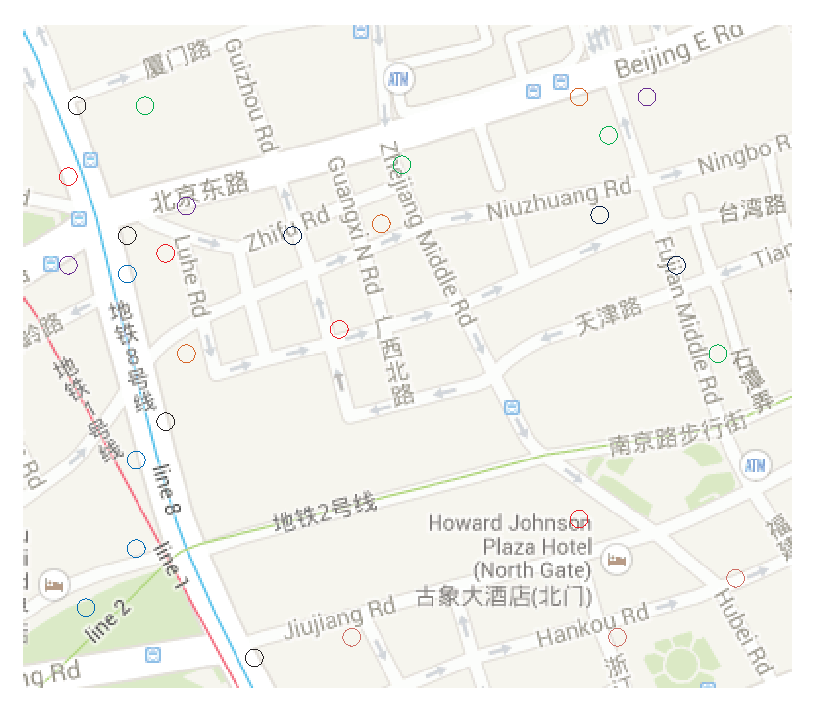
\includegraphics[width=0.85\columnwidth]{figures/fig-e-map-26.eps} \\
(a)
\end{tabular}
\begin{tabular}{cc}
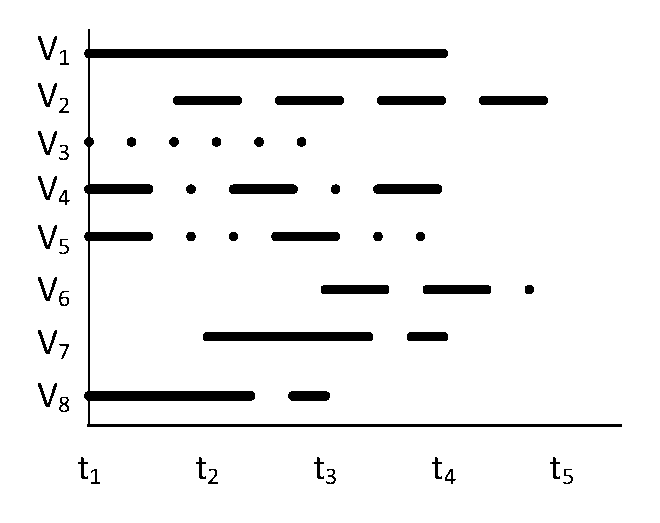
\includegraphics[width=0.45\columnwidth]{figures/fig-e-length-2.eps}&
\hspace {-0.1in}
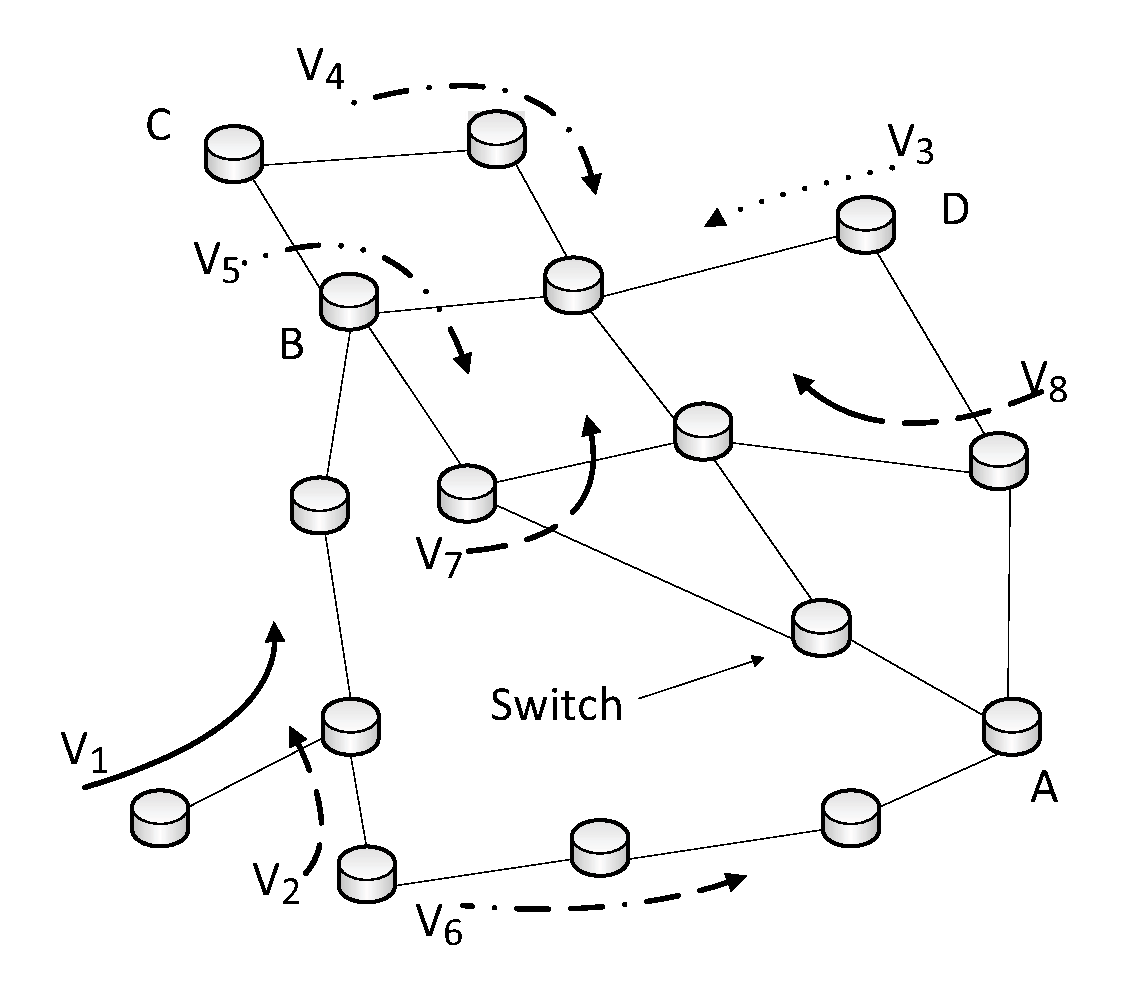
\includegraphics[width=0.45\columnwidth]{figures/fig-e-map-s-26-1.eps} \\
(b) & ~~~(c)
\end{tabular}
\caption{(a):上海市人民广场附近的场景图;(b):车辆的出现和离开时间;(c):(a)的简化图并保护车辆方向信息。} \label{fig8a}
  \end{center}
  % \vspace{-0.35in}
\end{figure}

\begin{figure} [t]
\begin{center}
\begin{tabular}{cc}
\includegraphics[width=0.5\columnwidth]{figures/fig-e-num-1.eps}&
\hspace {-0.2in}
\includegraphics[width=0.5\columnwidth]{figures/fig-e-num-2.eps} \\
(a) & (b)~~~
\end{tabular}
\begin{tabular}{c}
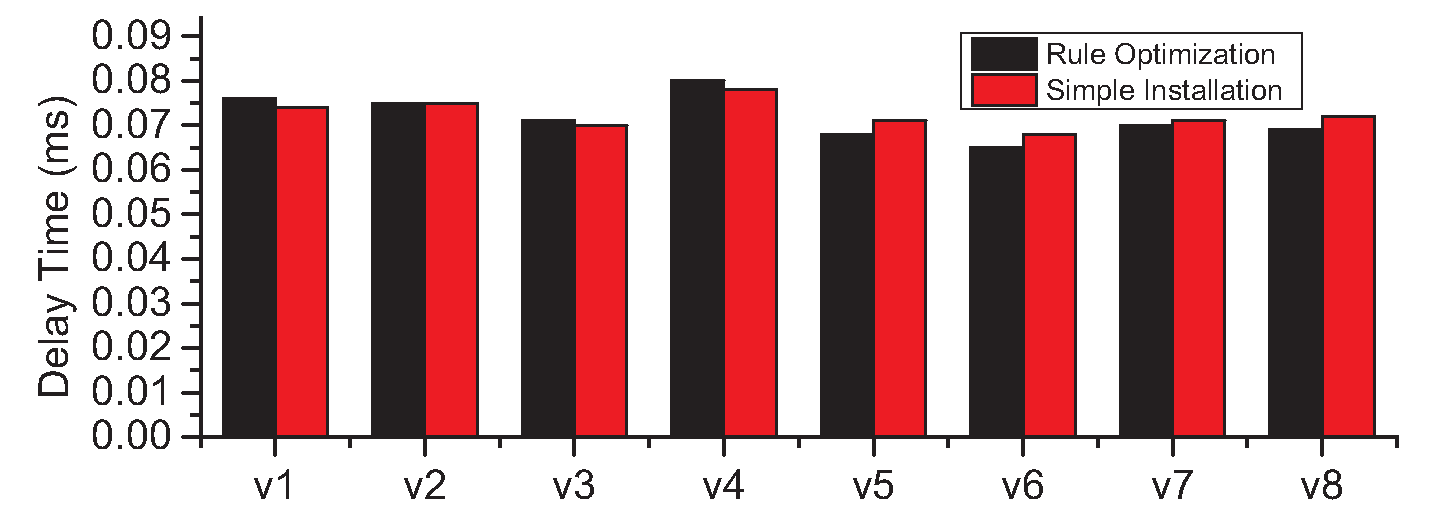
\includegraphics[width=0.9\columnwidth]{figures/fig-e-8bar-30.eps} \\
(c)
\end{tabular}
\caption{(a):两个策略的规则数量差异;(b):不同时刻的车辆数量;(c)两个策略的车辆延迟时间。 Simple Installation为对比方法,Rule Optimization为优化的流规则方法。} \label{fig8b}
  \end{center}
  % \vspace{-0.35in}
\end{figure}

\subsection{时延分析}


我们对两种模式(1对N和N对1)进行研究分析,并说明它们如何以不同方式影响结果。我们将规则数和延迟时间与对比方法进行比较,以表明它不会影响数据传输的性能。图~\ref{fig9}(a)显示N对1模式,即有多个车辆连接到一个监控摄像头($B$)。我们选择具有最长路径的$A$来评估延迟时间。对比方法需要在每个交换机上安装一个规则,并匹配源地址。对于所提的方法,从$B$传输到$A$的每个数据包都会修改包头(目标IP地址),然后转发到下一个交换机。图~\ref{fig9}(b)表明,随着交换机数量的增加,两种方法的延迟时间都变大,但没有显着差异。我们得出结论,优化的规则下发方法中的数据包修改过程不会影响性能。图~\ref{fig9}(c)显示了交换机的规则数量。红色(右侧)行表示节点$B$同时通过网络将数据流传输到每个节点的对比方法。每个交换机只需要一个规则基于$(*, B^{'})$ ($B^{'}$是多播地址)。黑色(左侧)线描述了优化的规则下发方法,该方法修改每个分支节点处的数据包目标地址,然后将数据包转发到给定端口。每个交换机只需要一个规则。


%We study two patterns (\textit{one-to-N} and \textit{N-to-one}) in details and show how they influence results differently. We compare the number of rules and the delay time with the baseline method to show that it does not affect the performance of data transmission. Fig.~\ref{fig9}(a) shows \textit{N-to-one} mode that there are multiple vehicles connecting to one surveillance camera ($B$). We pick $A$ that has the longest path to evaluate delay time. For the baseline method, it needs to install one rule at each switch with the match of source address. And for proposed approach, every packet transferred from $B$ to $A$ modifies the headers (destination IP address) at each switch and then forwards to the next switch. Fig.~\ref{fig9}(b) shows that, as the number of switches increases, delay time of both methods gets larger but with no statistically significant difference. We conclude that the packet modification process in improved rule installation does not influence performance. Fig.~\ref{fig9}(c) shows the number of rules at switches. The red (right side) line represents the baseline method that node $B$ transfers data flow across the network to every node at the same time. It only needs one rule at each switch with $(*, B^{'})$ ($B^{'}$ is the multicast address). The black (left side) line depicts improved rule installation approach that modifies the destination address at every branching node and then forwards the packets to given ports. It needs only one rule at each switch comparing to the the baseline method that requires multiple rules, the number of which equals to the data sources even they have the same destination. For example, the switches along $V_1$ to $B$ need two rules since $V_1$ also sends a request to $C$.

图~\ref{fig9}(d)显示1对N模式。其中车辆$V$同时连接多个摄像机($B, C, D$)。图~\ref{fig9}(e)显示了根据不同交换机数量的延迟时间。如果没有优化的规则下发,每个交换机的每个源节点都需要三个规则,$(B, *), (C, *), (D, *)$,这是源地址驱动模式(基于数据源转发数据包)。通过优化的规则下发,我们只需要一个规则,即每个交换机上的$(*, A)$,它仍然可以支持N对1模式。图~\ref{fig9}(f)显示了两种方法的规则数量。


%Fig.~\ref{fig9}(d) shows \textit{one-to-N} patterns where vehicle $V$ connects multiple cameras ($B, C, D$) at the same time. Fig.~\ref{fig9}(e) shows the delay time according to the different number of switches. Without improved rule installation, three rules are needed for each source node at each switch, $(B, *), (C, *), (D, *)$, which is a source-driven mode (forwarding packets based on data source). With improved rule installation, we need one rule only, i.e., $(*, A)$ at each switch and it can still support \textit{N-to-one} pattern. Fig.~\ref{fig9}(f) shows the number of rules of two methods.

我们从结果中得出两个结论。首先,分支节点处的数据包修改对数据传输的性能没有影响。其次,对于优化的规则下发的最佳情况(1对N),压缩后规则的数量与数据源的数量成比例。对于优化的规则下发的最坏情况(N对1),交换机的规则数量等于对比方法的规则数量。


%We draw two conclusions from the results. First, the modification of packets at branching nodes has no impact on the performance of data transmission. Second, for the best case of improved rule installation (\textit{one-to-N}), the number of reduced rules is proportional to the number of data sources. For the worst case of improved rule installation (\textit{N-to-one}), the number of rules at switches is equal to that of the baseline method.

%\begin{figure} [t]
%\begin{tabular}{cc}
%\includegraphics[width=0.5\columnwidth]{fig-e-1-30-a.eps}&\hspace{-0.05\columnwidth}
%\includegraphics[width=0.5\columnwidth]{fig-e-1-30-b.eps}\\
%(a) & (b)
%\end{tabular}
%\begin{tabular}{cc}
%\includegraphics[width=0.5\columnwidth]{fig-e-1-24.eps}&\hspace{-0.05\columnwidth}
%\includegraphics[width=0.5\columnwidth]{fig-e-3-24.eps} \\
%(c) & (d)
%\end{tabular}
%\begin{tabular}{cc}
%\includegraphics[width=0.5\columnwidth]{fig-e-2-24.eps}&\hspace{-0.05\columnwidth}
%\includegraphics[width=0.5\columnwidth]{fig-e-4-24.eps} \\
%(e) & (f)
%\end{tabular}
%\caption{Subfigure (a) shows a topology of \textit{N to 1} mode; (b) shows a topology of \textit{1 to N} mode; (c) shows delay time at different number of switches in (a); (d) shows delay time at different number of switches in (b); (e) shows number rules at different number of switches in (a); (f) shows number rules at different number of switches in (b)} \label{fig9}
%\end{figure}
\begin{figure*} [t]
\begin{center}
\scalebox{0.9}
{
\begin{tabular}{ccc}
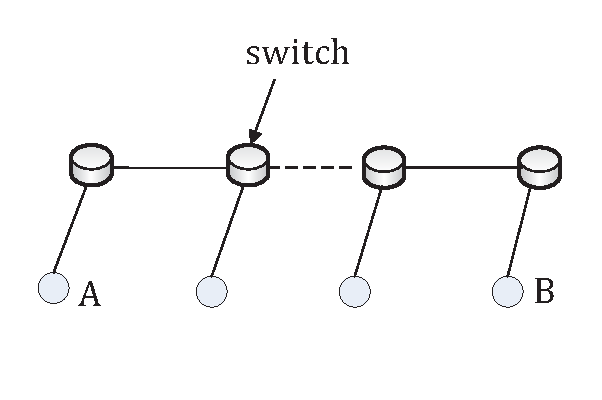
\includegraphics[width=0.33\columnwidth]{figures/fig-e-31-a.eps}&
\includegraphics[width=0.33\columnwidth]{figures/fig-e-1-24.eps}&\hspace{-0.1\columnwidth}
\includegraphics[width=0.33\columnwidth]{figures/fig-e-2-24.eps} \\
(a) & (b) & (c)
\\
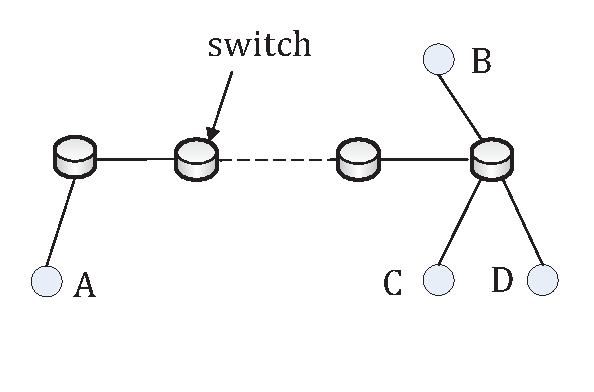
\includegraphics[width=0.33\columnwidth]{figures/fig-e-31-d.eps}&
\includegraphics[width=0.33\columnwidth]{figures/fig-e-3-24.eps}&\hspace{-0.1\columnwidth}
\includegraphics[width=0.33\columnwidth]{figures/fig-e-4-24.eps} \\
(d) & (e) & (f)
\end{tabular}
}
\caption{(a):N对1模式的拓扑;(b):对于(a)中不同交换机数量的延迟时间;(c):对于(a)中不同交换机数量的规则数量;(d):1对N模式的拓扑;(e):对于(d)中不同交换机数量的延迟时间;(c):对于(d)中不同交换机数量的规则数量。Simple Installation为对比方法,Rule Optimization为优化的流规则方法。} \label{fig9}
  \end{center}
% \vspace{-0.3in}
\end{figure*}


\section{本章小结}

本章针对车联网网络,提出软件定义车联网,SDIV的架构以及编程框架。其编程框架同时支持高级SDN程序以及响应式SDN程序。高级SDN程序可以主动编译成面向静态转发路径部分的数据通路。对于响应式SDN程序部分,则需要考虑对流规则进行压缩,即优化的流规则下发。实验结果可以看出,通过优化的流规则下发方法,生成的流规则数量降低。



